\documentclass{llncs}
%
%\documentclass[a4paper]{article}
\usepackage[UTF8]{ctex}
\usepackage{amsfonts}
\usepackage{amstext}
\usepackage{amsmath}
\usepackage{enumitem}
\usepackage{multirow}
\usepackage{graphicx}
\usepackage[center]{subfigure}
\usepackage{amssymb}
\usepackage{graphicx,amsmath} % Add all your packages here
\usepackage{subfigure}
\usepackage{algorithm}
\usepackage{algorithmic}
\renewcommand{\algorithmicrequire}{ \textbf{Input:}}
\renewcommand{\algorithmicensure}{ \textbf{Output:}}
\usepackage{url}
\usepackage{cite}
\usepackage{color}
\usepackage{pdfpages}
\usepackage{float}
\usepackage{booktabs}
\usepackage{fancyhdr}
\usepackage[colorlinks,linkcolor=black]{hyperref}
%页眉页脚
\pagestyle{fancy}
\lhead{}
\chead{}
\rhead{\bfseries 一课创业策划书}
\lfoot{From:ike team}
\cfoot{}
\rfoot{\thepage}
\renewcommand{\headrulewidth}{0.4pt}
\renewcommand{\footrulewidth}{0.4pt}
\fancypagestyle{plain}{
  \pagestyle{fancy}
}

%\usepackage{titlesec}
%公式编号含章节号
\makeatletter
\@addtoreset{equation}{section}
\makeatother
\renewcommand{\theequation}{\arabic{section}.\arabic{equation}}
\makeatletter
    \renewcommand{\thefigure}{\ifnum \c@chapter>\z@ \thechapter-\fi \@arabic\c@figure}
    \renewcommand{\thetable}{\ifnum \c@chapter>\z@ \thechapter-\fi \@arabic\c@table}
\makeatother
%章节号中文化
%\renewcommand\thesection{\chinese{section}、}
%\renewcommand\thesubsection{(\chinese{subsection})}
%\renewcommand\thesubsubsection{\arabic{subsubsection}}
%\usepackage\numberwithin{equation}{section}
%\titlespacing*{\section} {0pt}{3.5ex plus 1ex minus .2ex}{2.3ex plus .2ex}
\setcounter{secnumdepth}{3}
\setcounter{tocdepth}{3}
\begin{document}
\title{一课创业策划书}
\author{  }


\includepdf{data/cover.pdf}

\tableofcontents
\listoftables
\listoffigures

%\mainmatter
%book1
%\setcounter{page}{1}
\section{行业情况}
\subsection{行业概述}
现阶段中国在线教育的宏观发展环境一片利好.移动化和网络化的生活习养成、教育需求的上升以及技术的更新迭代为中国在线教育的发展注入源源不断的动力.从需求端角度来讲,用户对线上教育的认可度不断提升,对线上教育的种类和深度提出了更高的要求,同时随着知识扁平化的出现,用户对教学有效和教学体验的要求也将进一步推动在线教育发展。从供给端角度来看,大部分教师、教育机构及知识甲等都承担着教育盈余输出的角色,线上教育平台能够从技术、运营、推广、生源等方面提供辅助,而教师或机构的入驻能够进一步吸引生源从而带动平台收入,形成共赢局面。
但在实际市场上来看,还没有一家公司能够做到对在线教育、知识付费领域的主导地位,只是在某些细分领域有相应的领域领先者。而在线教育、知识付费领域的市场是巨大的,而且在逐年增长的过程中。
\subsection{政策说明}
\subsubsection{资金扶持}\

2014 年起,启动北京地区高校大学生创业优秀团队评选,给予优秀创业团队( 企业) 最多20 万元资助,并优先入驻大学生创业园。首批103个大学生创业优秀团队扶持资金1300 万元。2015 年预计资助400个优秀团队,扶持资金3200 万元。开展“北京高校大学生创新、创意、创业实践项目”支持,计划支持100个左右大学生创业团队、400个左右大学生创新创意、创业实践团队。

设立北京青年创业小额贷款担保基金,推出10 万元以下初创型企业小额贷款和500 万元以下成长型企业小额贷款项目。将个体工商户小额担保贷款最高担保额度和享受财政贴息最高贷款额度提高至20 万元,将小微企业担保贷款最高担保额度和享受财政贴息最高贷款额度提高至100 万元。同时,符合条件的北京市合同期满未就业大学生村官和本市低保、低收入家庭高校毕业生不提供任何担保就申请贷款。

\subsubsection{创业载体建设}\

中国人民大学大学生创业园,凡为中国人民大学注册在校生、应届毕业生及已毕业(两年内)尚未就业的大学生,经中国人民大学在职教师推荐,均可申请入驻学生创业园,包括本科生、硕士生、博士生。

\subsubsection{创业教育培训}\

\paragraph{教育形式多种多样}\

先后在中国人民大学等7 所高校开设创业培训服务基地校,符合条件的高校毕业生可享受创业导师辅导。拥有北京市户籍的大学生可根据自身创业需求,到指定创业培训定点机构参加一次免费创业培训。

\paragraph{辅导专家团队不断组建}\

2009 年,北京首家“大学生创业指导中心”在北京交通大学挂牌。2014 年,启动北京高校示范性创业中心建设工作,用三年时间建设40个左右示范性高校创业指导中心。首批中国农业大学、首都师范大学等24所高校入选,分别给予50万元建设经费支持。

\paragraph{创新创业竞赛蓬勃发展}\

2000 年起,北京开始举办首都大学生创业计划竞赛,80 余所高校超过50 万大学生直接或间接参与创业竞赛活动,目前已举办8 届。2013 年起,每年举办北京市大学生创业设计竞赛,搭建大学生创业设计成果交流展示平台。2014 年,北京市大学生创业引领计划之“东升杯”大学生创业大赛正式启动,优胜者将可获得现金奖励、免费办公场所、全方位孵化服务等奖项,总价值200余万。(“互联网+“创业大赛。)

\subsection{用户人群}
用户人群标签:
\begin{figure}[H]
	\centering
	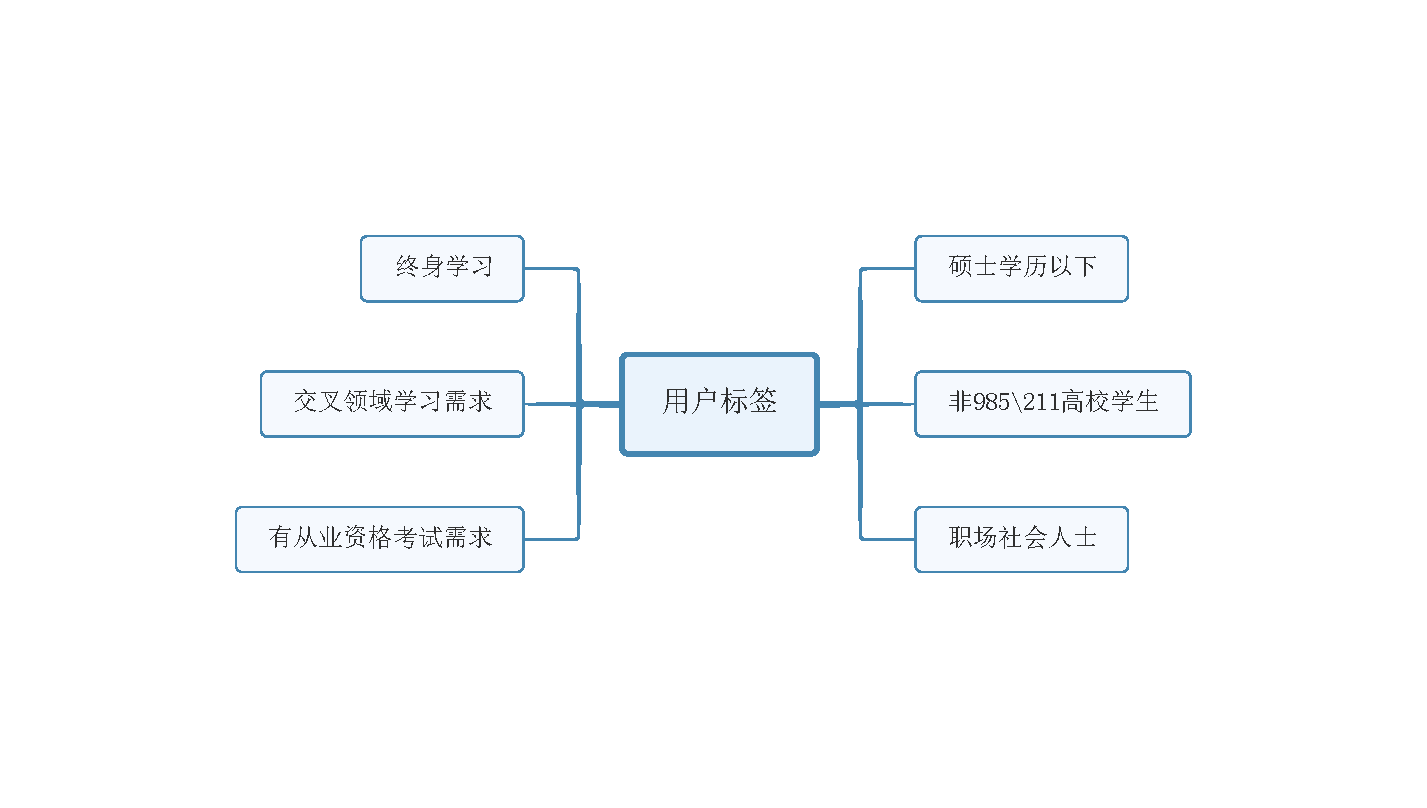
\includegraphics[width=0.9\columnwidth]{figures/user_label}
	%  \setlength{\abovecaptionskip}{0pt}
	%  \setlength{\belowcaptionskip}{-20pt}
	\caption{用户人群标签}
	\label{fg:user_label}
\end{figure}

\subsection{未来发展}
参考以下数据:
\begin{figure}[H]
	\centering
	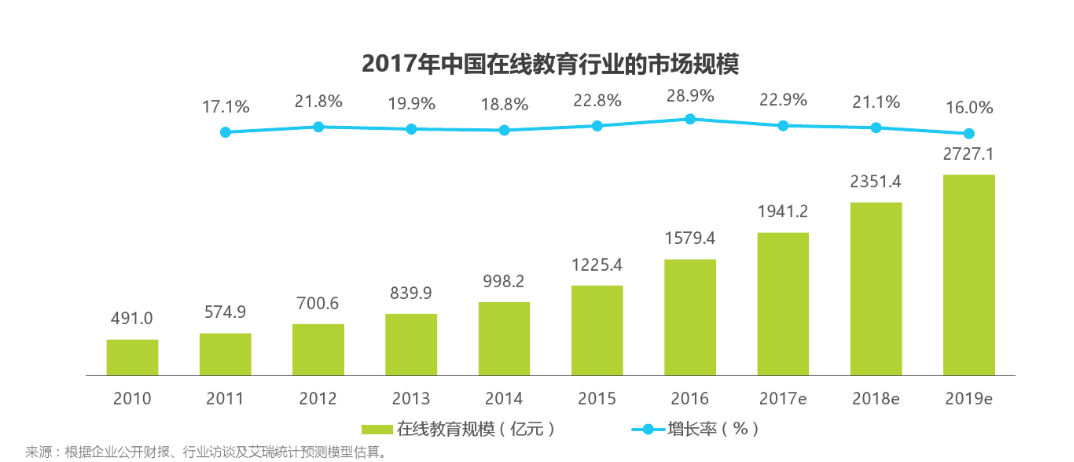
\includegraphics[width=0.9\columnwidth]{figures/2017online_education}
	%  \setlength{\abovecaptionskip}{0pt}
	%  \setlength{\belowcaptionskip}{-20pt}
	\caption{2017年在线教育行业的市场规模}
	\label{fg:2017online_education}
\end{figure}

\begin{figure}[H]
	\centering
	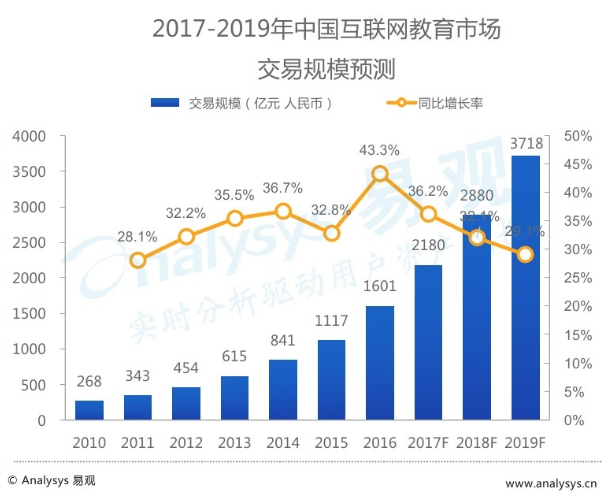
\includegraphics[width=0.9\columnwidth]{figures/2017_2019internet_education}
	%  \setlength{\abovecaptionskip}{0pt}
	%  \setlength{\belowcaptionskip}{-20pt}
	\caption{2017-2019年中国互联网教育市场交易规模预测}
	\label{fg:2017_2019internet_education}
\end{figure}

\begin{figure}[H]
	\centering
	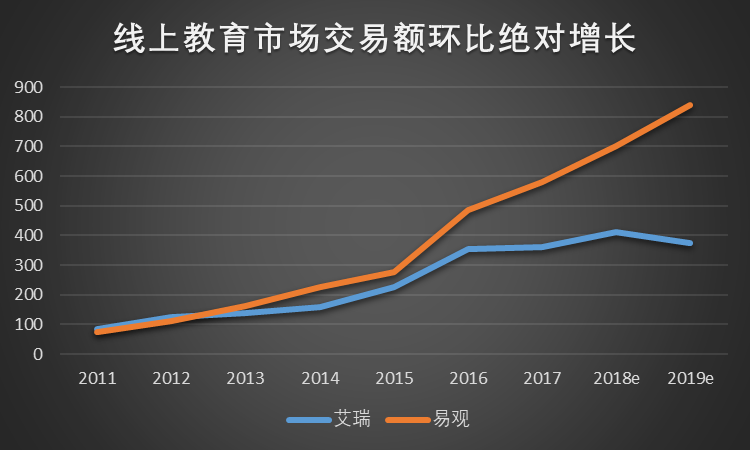
\includegraphics[width=0.9\columnwidth]{figures/online_education}
	%  \setlength{\abovecaptionskip}{0pt}
	%  \setlength{\belowcaptionskip}{-20pt}
	\caption{线上教育市场交易额环比绝对增长}
	\label{fg:online_education}
\end{figure}

\subsubsection{宏观环境利好}\

互联网+教育、教育信息化及AI+教育等利好政策频出;

网络经济上行,网络化和移动化生活习惯养成;

社会供需失衡,随着中产阶级崛起,人们付费意识觉醒,教育需求和教育消费迎来升级;

互动直播、大数据、人工智能等技术提升线上教育教学体验;

根据《新媒体蓝皮书:中国新媒体发展报告(2018)》,到2017年底,知识付费用户达到1.88亿人,比2016年增长了102.2%。而华菁证券的研报推断,到2020年知识付费将会有2亿人群、45%付费率、360元ARPU值,行业总收入规模达到320亿。

\subsubsection{知识需求端市场旺盛}\

在线教育用户规模持续扩张,在线教育的市场认可度逐渐提升,对线上课程的广度和内容深度要求提升;

终身学习和对交叉领域知识的需求增加测试用户需要学习的阶段不断延长;

用户重视学习的有效性,并对线上学习体验不断提出新的需求。

\subsubsection{知识供给端输出盈余}\

传统教师或中小型教育机构转型线上教育成本高且经验缺乏;
独立知识分享者可提供短平快的知识输出,但是在生源和推广方面有待加强。
















%行业情况
%\section{市场方案}
\subsection{市场需求调研方式}

企业与市场的关系是不可分割的。简单来说:企业是为了市场的需要而存在的,也可以说企业是服务于市场的;市场有着不同的需求,而企业为了满足市场的种种需求而发展壮大。在进行新产品暨课程开发前,本公司将充分做好市场需求调研,在考虑公司今后长远发展规划的基础之上寻求需求最大最具市场价值的发展方向,这一方面应该后期将专门由公司知识管理部负责。注意调研的有效性及专业性,可参考的一些方式:

\paragraph{大数据调研}\

从易观、艾瑞等专业大数据平台或其他方面获取数据,分析目前市场状况及未来发展趋势并作出市场发展判断,从而选定新课程研发方向。

\paragraph{线下调研}\

通过对线下机构及线上用户的需求调研,根据调研结果有针对性地开展接下来的产品研发方向选择工作。此方法能有效增强与用户的交互性并且获得数据更为直接可靠。

\paragraph{知识管理规划}\

依据公司战略发展目标,与具体可实施性,在与课程运营部密切合作沟通的同时,把握前沿知识管理与知识创造的方法,同时按照公司知识管理方法指导实施,协助修正市场调研得出的课程研发方向。

\subsection{市场需求预调研}
如图\ref{fg:B2B2C2017}:
\begin{figure}[H]
	\centering
	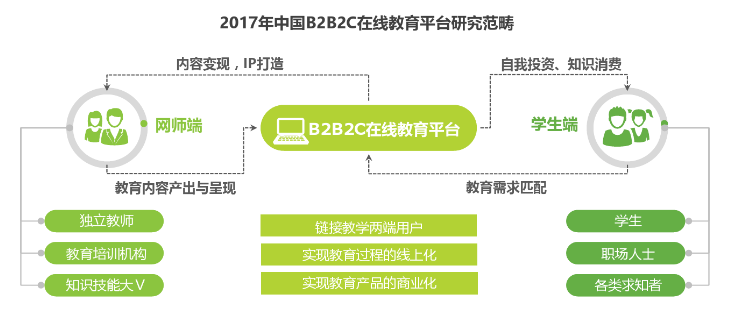
\includegraphics[width=0.9\columnwidth]{figures/B2B2C2017.png}
	%  \setlength{\abovecaptionskip}{0pt}
	%  \setlength{\belowcaptionskip}{-20pt}
	\caption{2017年中国B2B2C在线教育平台研究范畴}
	\label{fg:B2B2C2017}
\end{figure}

\paragraph{知识提供方}\

知识变现的需要,特别是受过高等教育的人,他们会有很多隐性知识的储备,但没有渠道输出,没有可以获得利益的渠道。或者他们有这样的渠道,但是收到的效果并不好。

\paragraph{知识需求方}\

知识改变命运,现代人对终身教育的需要,不断学习的理念的深入人心,对个人技能的补充,对大学所学专业内容的不适应,对深入学习的需要。

\begin{figure}[H]
	\centering
	
\includegraphics[width=0.9\columnwidth]{figures/relationship}
	%  \setlength{\abovecaptionskip}{0pt}
	%  \setlength{\belowcaptionskip}{-20pt}
	\caption{两者的关系}
	\label{fg:relationship}
\end{figure}


\subsection{销售模式}

\subsubsection{前期}\

寻找校园代理,通过校园代理来拓宽教师来源渠道,在系统开发的同时,进行课程的录制,课程录制的方向是:先进行市场调查,市场调查的依据是询问线下教育行业人士,然后针对性的进行课程录制,课程销售交给线下教育行业人士,通过获得收益分成的方式吸引合作者。

\begin{figure}[H]
	\centering
	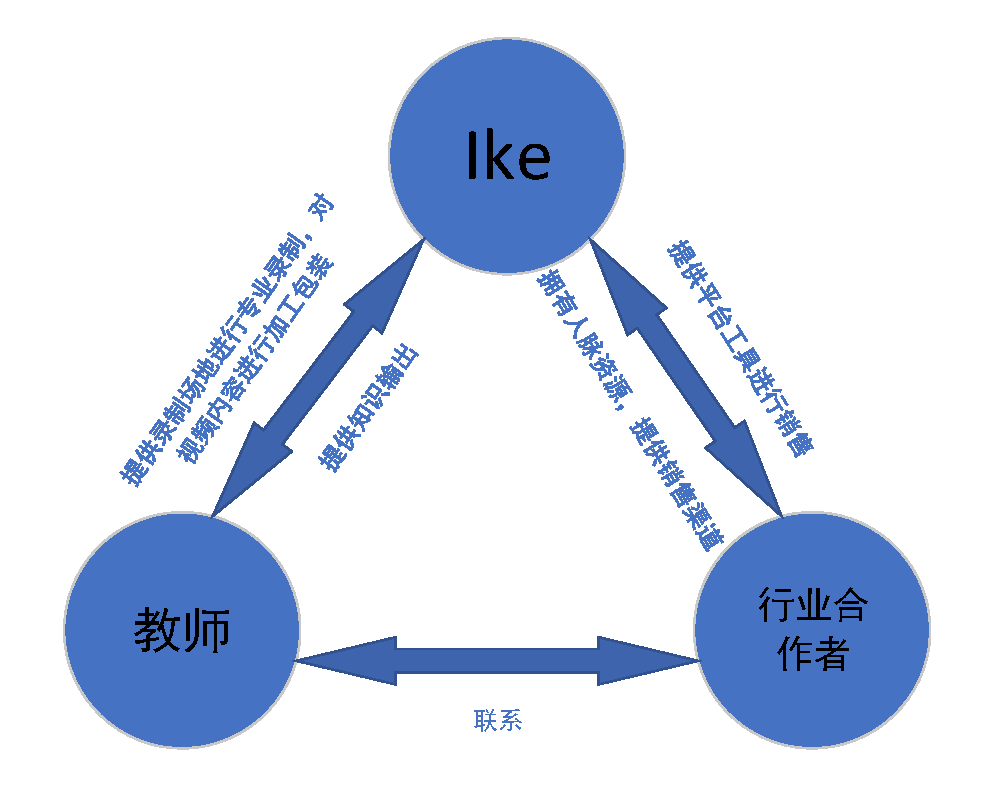
\includegraphics[width=0.9\columnwidth]{figures/partnership}
	%  \setlength{\abovecaptionskip}{0pt}
	%  \setlength{\belowcaptionskip}{-20pt}
	\caption{合作关系}
	\label{fg:partnership}
\end{figure}

\subsubsection{中期}\

当前期盈利模式获得一定收益之后,增加销售部,销售部组成人员主要来源于社会招聘,通过市场上的有经验的销售人员,通过销售人员来留住客户,同时,课程录制开始逐渐完善平台总体课程框架,开始录制大学专业介绍,初步拥有品牌知名度;对平台课程视频资源的重新整合加工,二次销售给市场,加大融资。部分课程免费开放吸引流量打开市场。

\subsubsection{后期}\

独立营业模式超过现有的教育平台,有足够强壮的基础课程体系后,进军K12领域并寻求与地方政府的合作,通过低价格的形式将课程卖给或者送给偏远贫困地区学生,打响平台品牌;与电商合作;增加知识管理部门,对平台已有的三大知识储存载体,进行知识的提炼,知识元的加工,转化的二次加工产品输出,公司主要盈利和影响力将来源于此。

\subsection{产品定价}

产品定价是产品在市场中占据主动的前提,适当的产品定价能帮助企业在激烈的市场竞争中占得先机。本公司运营产品目前主要为课程成品,定价时主要考虑课程的内容价值以及目前在线教育市场的供求关系,在兼顾消费者的购买力基础之上,通过一定算法得出产品最适宜的市场定价。目前针对公司运营时期变化主要采取三种定价方式。

\subsubsection{质量加成定价}\

课程研发之初,本公司将充分考虑课程知识、教师水平、内容难获取程度等多发面因素确保产品质量。产品定价时,在考虑目前市场价的基础之上,针对本产品的质量优势进行一定的加权处理,同时综合考虑教师知名度、教师背景、教师形象等可能对课程销售产生影响的因素,最终确定本课程定价。

\subsubsection{市场导向定价}\

在课程销售经过一定时间之后,参考市场销售反馈情况,课程的定价需要根据市场反馈作出一定调整。初步考虑将产品的浏览量与购买量的比值关系作为市场反馈的一个表现因素,根据市场导向最终确定课程的定价调整计划。

\subsubsection{竞争导向定价}\

在课程销售的后期,考虑同类型企业将会越来越多出现,市场竞争也将会越来越激烈。激烈的市场竞争之中要想取得优势就需要看清形势,针对当前同类产品竞争情况作出针对性价格调整,以在竞争中保持优势地位。




%市场方案
%\section{产品运营}
\subsection{产品简要介绍}\

\subsubsection{产品类型}\

全品类半开放式的知识付费平台——以教学视频以及配套音频,配套习题和配套资料为主。

\paragraph{全品类}\

单一品类竞争激烈,而且市场发展受限,而在线上教育领域并不存在所谓的“全部都做反而什么都做不好”的顾虑,因为平台只能做筛选教师工作,平台本身并不是知识的输出者,我们面向社会所有人招收教师来源,我们要做的是课程质量评价体系,保障课程质量,线上教育主要吸引人的是它便宜的价格。

\paragraph{半开放式}\

针对市面上已有的两种线上教育平台找老师的模式的综合与改进,一种是全开放式的,也就是拥有教师端的平台,平台通过对知识输出端的全开放,老师通过注册教师资格,自主上传教学课程;一种是全封闭式的,没有教师端,老师全靠课程运营联系,课程经审核规划后上线平台。

而半开放式平台是只开放教师联系的端口,老师不能直接上传课程,方便有知识变现需求的人联系平台,同时我们也要求课程运营联系老师,双管齐下,平台以此获取教师来源,从而筛选教师,教师需要遵守公司对课程录制的要求进行录课。
\vfill
% Table generated by Excel2LaTeX from sheet 'Sheet1'
\begin{table}[H]
  \centering
  \caption{运营模式对比}
    \begin{tabular}{|r|p{8.89em}|c|}
    \hline
    \textcolor[rgb]{ .298,  .282,  .239}{} & \textcolor[rgb]{ .298,  .282,  .239}{优点} & \multicolumn{1}{p{14.055em}|}{\textcolor[rgb]{ .298,  .282,  .239}{缺点}} \\
    \hline
    \multicolumn{1}{|r|}{\multirow{4}[2]{*}{\textcolor[rgb]{ .298,  .282,  .239}{全开放式平台}}} & \multirow{4}[2]{*}{\textcolor[rgb]{ .298,  .282,  .239}{课程覆盖速度快}} & \multicolumn{1}{p{14.055em}|}{\textcolor[rgb]{ .298,  .282,  .239}{1.管理混乱}} \\
          & \multicolumn{1}{c|}{} & \multicolumn{1}{p{14.055em}|}{\textcolor[rgb]{ .298,  .282,  .239}{2.课程质量很难保障}} \\
          & \multicolumn{1}{c|}{} & \multicolumn{1}{p{14.055em}|}{\textcolor[rgb]{ .298,  .282,  .239}{3.平台后期知识管理实施困难}} \\
          & \multicolumn{1}{c|}{} & \multicolumn{1}{p{14.055em}|}{\textcolor[rgb]{ .298,  .282,  .239}{4.课程盈利较少,只是抽取平台使用费}} \\
    \hline
    \multicolumn{1}{|r|}{\multirow{3}[2]{*}{\textcolor[rgb]{ .298,  .282,  .239}{全封闭式平台}}} & \textcolor[rgb]{ .298,  .282,  .239}{1.课程质量平台可控制} & \multicolumn{1}{p{14.055em}|}{\textcolor[rgb]{ .298,  .282,  .239}{1.效率低}} \\
          & \textcolor[rgb]{ .298,  .282,  .239}{2.后期知识管理方便} & \multicolumn{1}{p{14.055em}|}{\textcolor[rgb]{ .298,  .282,  .239}{2.课程制作周期长}} \\
          & \textcolor[rgb]{ .298,  .282,  .239}{3.课程盈利较多} & \multicolumn{1}{p{14.055em}|}{\textcolor[rgb]{ .298,  .282,  .239}{3.课程覆盖速度慢}} \\
    \hline
    \multicolumn{1}{|r|}{\multirow{5}[2]{*}{\textcolor[rgb]{ .298,  .282,  .239}{半开放式平台}}} & \textcolor[rgb]{ .298,  .282,  .239}{1.课程质量平台可控制} & \multicolumn{1}{c|}{\multirow{5}[2]{*}{\textcolor[rgb]{ .298,  .282,  .239}{暂无}}} \\
          & \textcolor[rgb]{ .298,  .282,  .239}{2.后期知识管理方便} &  \\
          & \textcolor[rgb]{ .298,  .282,  .239}{3.课程制作周期短} &  \\
          & \textcolor[rgb]{ .298,  .282,  .239}{4.课程覆盖速度快} &  \\
          & \textcolor[rgb]{ .298,  .282,  .239}{5.课程盈利较多} &  \\
    \hline
    \end{tabular}%
  \label{tab:yymsdb}%
\end{table}%


\subsubsection{产品核心}\

课程内容为核心,技术为工具。

前期通过与老师签订版权归属协议,拥有对高等教育高质量的、公司具有完全版权的课程,后期通过对课程的二次加工,整合课程,对现有知识形成一个知识创造。给用户个性化推荐课程套餐,而这种课程二次加工后的课程套餐,对于拥有课程完全版权的公司来说成本低且易操作。

\subsubsection{产品市场切入点}\

K12之后的线上教育。如:

成人教育:信息技术;平面设计;

高等教育:高等数学;

技能培训:化妆课;插花;

资格考试:司法考试;公务员考试。

原因:首先是因为K12已经有了行业巨头与行业标准(学而思),其次是考虑到对社会的影响来说,真正助推中国社会对人才的需求的,不是K12,而是成人教育。但另一方面,我们并不是完全放弃K12,我们是全品类的知识付费平台,为了迎合市场刚需和与政府的合作,平台的课程课程将会覆盖到K12,在这方面的课程质量保障,只需要直接联系学而思现役有经验的老师录制课程,然后我们以较低价格提供给市场或者免费送课(价格战)。

\subsection{课程运营选择方向}
\subsubsection{录课形式}\

作为全品类的平台,全品类不仅体现在课程种类上,也体现在录课形式上,主要分为两种录课形式。举现有的市场平台的例子,万题库,它是只做直播课程的全开放平台,但直播课并没有达到预期的效果,甚至还不如录播课,参考艾瑞咨询:2018年1月中国在线教育平台用户大数据报告:腾讯课堂数据篇

\begin{figure}[H]
	\centering
	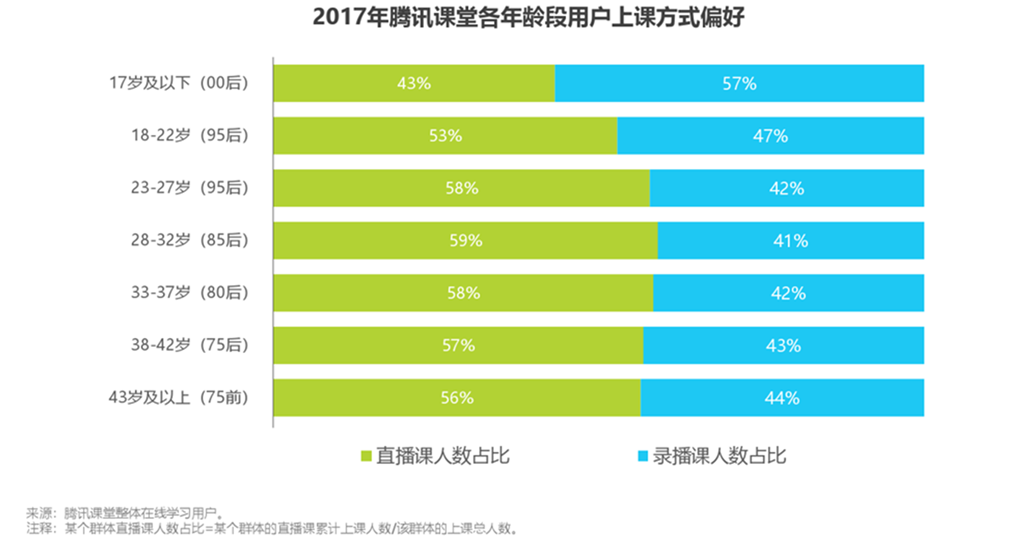
\includegraphics[width=0.9\columnwidth]{figures/tecent_couse.png}
	%  \setlength{\abovecaptionskip}{0pt}
	%  \setlength{\belowcaptionskip}{-20pt}
	\caption{2017年腾讯课堂各年龄用户上课方式偏好}
	\label{fg:tecent_couse}
\end{figure}

这张图我们可以看到,并不是像万题库所描述的那样,直播课对于录播课来说具有压倒性优势,所以只做直播课就好了,而是我们看到越年轻的人群越喜欢录播课,他们更适应快捷的获取知识的方式,对他们来说直播听课花费的时间太高。另一方面,直播课还存在很多问题,比如现阶段直播间的普遍问题,主播有事暂离,只能空闲等待,在直播课时,若老师临时演板,也就只能等老师写完,这段时间是接受知识的空白区。老师语速慢也不能快进,在时间上效率较低。而且直播所推崇的实时互动只局限于小用户量,人数一旦达到一定数量,实时互动的效果就会大打折扣。所以,直播课和录播课我们都要有,直播课有它在学习效果上的优势,而录播课则也有它受欢迎的人群。对于市场需求来说二者相对平均,这在某种程度上再一次验证了坚持全品类的正确性。

\subsubsection{课程内容}\

\paragraph{市场受欢迎的课}\

作为商业公司,首先以盈利为主,公司的前期的成本回收主要依靠于此。公司将会在课程选择前做好市场调查,而市场调查的主要手段包括各数据平台年报数据分析,与对业内人生访谈,对知乎的调研。

\paragraph{为形成公司完整课程体系的课}\

为了提高公司的竞争潜力与核心竞争力,需要尽快完善课程体系,首先遍历大学大类课程,比如经济金融课程体系化特训班,拿到完全版权后,课程将被按大学课程拆分成微观经济学部分,宏观经济学部分等单独售卖,之后通过销售反馈销售情况,再考虑是否就受欢迎课程进行重新录制,提高该类课程质量。当公司大量盈利之后将遍历精细化所有小门类课程,以做出品牌效应。

\paragraph{为和政府合作提高社会影响力的课}\

首选K12.。

\subsubsection{其他非视频形式}\

\paragraph{课程配套资料}\

课程配套资料,可以通过学生自己上传,公司整理后可出书出售。

\paragraph{课程音频}\

为了满足部分课程内容对于图像资料的需求度不高,和部分用户有只听音频的需求,公司的课程需要有单独的音频部分可以供用户体验。

\paragraph{课程配套习题}\

后期上线的功能,主要在于评价学生知识掌握情况,与后期习题册出版。

\subsection{课程制作流程图}
课程制作流程如下:
\begin{figure}[H]
	\centering
	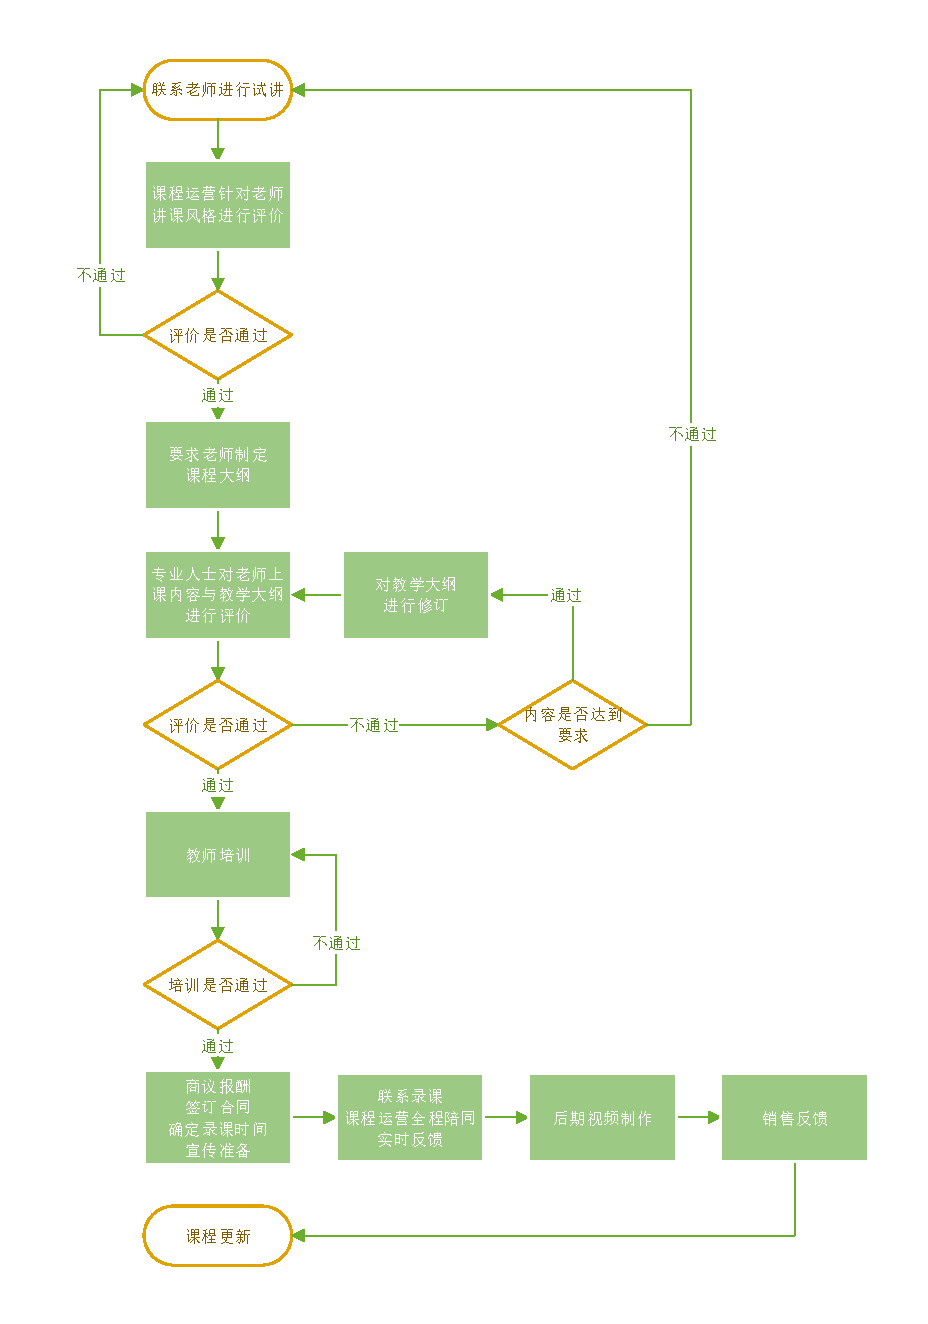
\includegraphics[width=0.9\columnwidth]{figures/couse_process}
	%  \setlength{\abovecaptionskip}{0pt}
	%  \setlength{\belowcaptionskip}{-20pt}
	\caption{课程制作流程图}
	\label{fg:couse_process}
\end{figure}

\subsection{课程功能实现}\

\paragraph{奖励机制}\

通过用户课程笔记的上传,后台会评价出最优的笔记,分享给所有的用户,上传者该课程免费。

\paragraph{评价系统}\

点赞量高、内容质量好的评价会优先显示在顶端(参考网易云音乐的评价系统)。

\paragraph{学友系统(后期可以考虑实现)}\

学生之间可以加好友加关注,一起学习,互相留言探讨问题,也相当于借鉴现在软件系统行业发展的趋势,社交是用户黏度的另一种提升方式。参考各类游戏、实用软件,大部分都植入了社交系统,因为人是群居动物,具有随大流的趋势。

\paragraph{答疑系统,师生交互(成熟后实现)}\

可选取专门时间段开教师直播答疑课,解决学员在学习过程中遇到的典型性问题。问题来源可以是专门学员反馈(课后留专门邮箱接收),也可以是讨论区(类似学友系统)反馈,也可以是老师想到的典型问题。

\subsection{课程质量控制}
\subsubsection{课程分类体系}\

初步方案:

\begin{figure}[H]
	\centering
	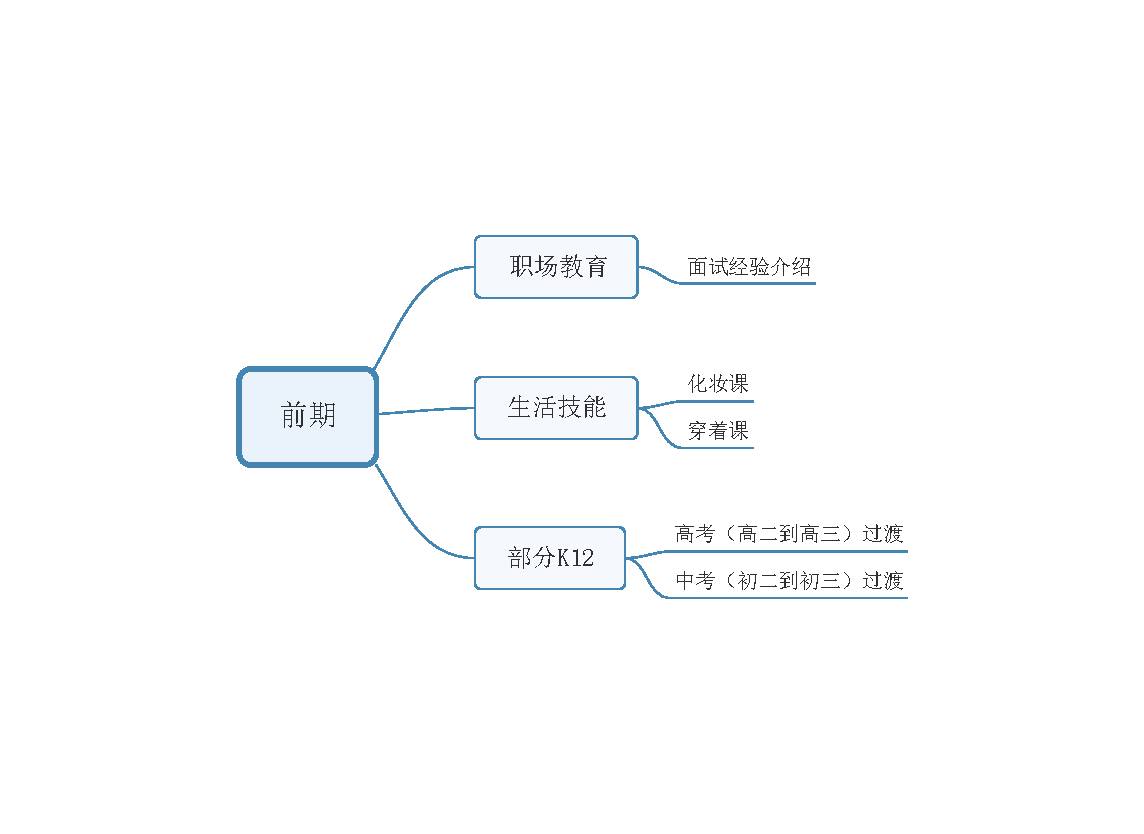
\includegraphics[width=0.9\columnwidth]{figures/prophase_development}
	%  \setlength{\abovecaptionskip}{0pt}
	%  \setlength{\belowcaptionskip}{-20pt}
	\caption{课程分类体系}
	\label{fg:prophase_development}
\end{figure}

最终方案:参考第一章第7节第2小节长期目标图\ref{fg:aft_development}

\subsubsection{教师来源}\

\paragraph{老师客户}\

在平台主动联系公司的老师,这也是公司主要想发展的方面,前期通过宣传,长期通过做口碑来实现这一点。

\paragraph{高校学生}\

公司的创业团队覆盖了北京最好的几所高校,据我们了解,我们身边想要知识变现的人很多,公司可以直接通过公司管理层或者员工联系同学校的学生资源。使用我们创业团队的优势,收集北京各个院校的各个学院的情况,找到有空余时间的学生。另一方面,对于学生来说公司可以给于的报酬足够吸引他们来将知识变现。而阻碍合作的有两个主要的原因,一是没有时间,二是路程。

\paragraph{线下机构教师}\

成熟机构有经验的老师,技能培训以及从业资格考试类。

\subsubsection{教师要求}\

\paragraph{试讲环节}\

试讲评分项目:
% Table generated by Excel2LaTeX from sheet 'Sheet1'
\begin{table}[H]
  \centering
  \caption{试讲评分项目}
    \begin{tabular}{|p{16.165em}|r|}
    \hline
    \textcolor[rgb]{ .298,  .282,  .239}{试讲评分项目} & \multicolumn{1}{p{16.945em}|}{\textcolor[rgb]{ .298,  .282,  .239}{分数(10分制)}} \\
    \hline
    \textcolor[rgb]{ .298,  .282,  .239}{1.所讲内容是否正确(基础)} & \textcolor[rgb]{ .298,  .282,  .239}{} \\
    \hline
    \textcolor[rgb]{ .298,  .282,  .239}{2.语速是否适当} & \textcolor[rgb]{ .298,  .282,  .239}{} \\
    \hline
    \textcolor[rgb]{ .298,  .282,  .239}{3.讲课逻辑是否清晰} & \textcolor[rgb]{ .298,  .282,  .239}{} \\
    \hline
    \textcolor[rgb]{ .298,  .282,  .239}{4.习惯语是否太多,呃嗯等} & \textcolor[rgb]{ .298,  .282,  .239}{} \\
    \hline
    \textcolor[rgb]{ .298,  .282,  .239}{5.是否用太多的专业术语让人不好理解} & \textcolor[rgb]{ .298,  .282,  .239}{} \\
    \hline
    \textcolor[rgb]{ .298,  .282,  .239}{6.准备是否充分,知道自己接下来要讲什么} & \textcolor[rgb]{ .298,  .282,  .239}{} \\
    \hline
    \textcolor[rgb]{ .298,  .282,  .239}{7.声音是否洪亮} & \textcolor[rgb]{ .298,  .282,  .239}{} \\
    \hline
    \textcolor[rgb]{ .298,  .282,  .239}{8.录课形象是否合适} & \textcolor[rgb]{ .298,  .282,  .239}{} \\
    \hline
    \end{tabular}%
  \label{tab:sjpfxm}%
\end{table}%


\paragraph{第三方评价环境}\

讲课内容评价
% Table generated by Excel2LaTeX from sheet 'Sheet1'
\begin{table}[H]
  \centering
  \caption{讲课内容评价}
    \begin{tabular}{|p{14.335em}|r|}
    \hline
    \textcolor[rgb]{ .298,  .282,  .239}{讲课内容具体评价} & \multicolumn{1}{p{12.665em}|}{\textcolor[rgb]{ .298,  .282,  .239}{分数(10分制)}} \\
    \hline
    \textcolor[rgb]{ .298,  .282,  .239}{1.所讲内容是否正确(专业角度)} & \textcolor[rgb]{ .298,  .282,  .239}{} \\
    \hline
    \textcolor[rgb]{ .298,  .282,  .239}{2.所讲知识是否足够前沿} & \textcolor[rgb]{ .298,  .282,  .239}{} \\
    \hline
    \textcolor[rgb]{ .298,  .282,  .239}{3.教学大纲内容设计是否合理} & \textcolor[rgb]{ .298,  .282,  .239}{} \\
    \hline
    \textcolor[rgb]{ .298,  .282,  .239}{4.教学大纲时间分配是否得当} & \textcolor[rgb]{ .298,  .282,  .239}{} \\
    \hline
    \textcolor[rgb]{ .298,  .282,  .239}{5.作为专业学生,您是否想听他/她的课} & \textcolor[rgb]{ .298,  .282,  .239}{} \\
    \hline
    \end{tabular}%
  \label{tab:nrpf}%
\end{table}%


\subsubsection{教师合同}\

教学兼职合同

录播教学课程合同/直播教学课程合同

版权归属协议(许可使用作品目录)

买断教师一定时间内线上同类型课程录制权利

\subsubsection{课程制作周期}\
以微观经济学为例:
% Table generated by Excel2LaTeX from sheet 'Sheet1'
\begin{table}[H]
  \centering
  \caption{课程更新周期(例)}
    \begin{tabular}{|p{5.165em}|p{6.61em}|p{8.165em}|p{4.055em}|}
    \hline
    \textcolor[rgb]{ .298,  .282,  .239}{课程类型} & \textcolor[rgb]{ .298,  .282,  .239}{课程名称} & \textcolor[rgb]{ .298,  .282,  .239}{一年内是否需要更新} & \textcolor[rgb]{ .298,  .282,  .239}{更新周期} \\
    \hline
    \textcolor[rgb]{ .298,  .282,  .239}{大学专业课} & \textcolor[rgb]{ .298,  .282,  .239}{微观经济学} & \textcolor[rgb]{ .298,  .282,  .239}{否} & \textcolor[rgb]{ .298,  .282,  .239}{2-3年} \\
    \hline
    \end{tabular}%
  \label{tab:kcgxzq}%
\end{table}%


\subsection{成本投入}
\subsubsection{兼职教师报酬}\

兼职教师报酬为:
% Table generated by Excel2LaTeX from sheet 'Sheet1'
\begin{table}[H]
  \centering
  \caption{兼职教师报酬}
    \begin{tabular}{|p{5.165em}|p{8.665em}|p{6.835em}|p{5.5em}|}
    \hline
    \textcolor[rgb]{ .298,  .282,  .239}{教师类型} & \textcolor[rgb]{ .298,  .282,  .239}{讲课内容} & \textcolor[rgb]{ .298,  .282,  .239}{形式} & \textcolor[rgb]{ .298,  .282,  .239}{价格} \\
    \hline
    \textcolor[rgb]{ .298,  .282,  .239}{大学博士} & \textcolor[rgb]{ .298,  .282,  .239}{高等教育、司法考试} & \textcolor[rgb]{ .298,  .282,  .239}{直播+录播} & \textcolor[rgb]{ .298,  .282,  .239}{1000+/h} \\
    \hline
    \textcolor[rgb]{ .298,  .282,  .239}{大学硕士} & \textcolor[rgb]{ .298,  .282,  .239}{高等教育、考研、基础课程} & \textcolor[rgb]{ .298,  .282,  .239}{教研+直播+录播} & \textcolor[rgb]{ .298,  .282,  .239}{400-1000/h} \\
    \hline
    \textcolor[rgb]{ .298,  .282,  .239}{大学本科} & \textcolor[rgb]{ .298,  .282,  .239}{K12} & \textcolor[rgb]{ .298,  .282,  .239}{录播} & \textcolor[rgb]{ .298,  .282,  .239}{500/h} \\
    \hline
    \textcolor[rgb]{ .298,  .282,  .239}{社会人士} & \textcolor[rgb]{ .298,  .282,  .239}{公务员考试、化妆课;兴趣课技能课考证课} & \textcolor[rgb]{ .298,  .282,  .239}{录播} & \textcolor[rgb]{ .298,  .282,  .239}{1000/h} \\
    \hline
    \end{tabular}%
  \label{tab:jzlsbc}%
\end{table}%


\subsubsection{场地需求}\

\paragraph{直播课场地}\

场地要求:
\begin{itemize}
  \item 场地大小:20平米
  \item 录课环境安静(必要时贴吸音泡沫)
  \item 录课时空调声音不能影响录课效果
\end{itemize}


\paragraph{录播课场地}\

场地要求:
\begin{itemize}
  \item 场地大小:5-6平米
  \item 录课环境安静(必要时贴吸音泡沫)
  \item 录课时空调声音不能影响录课效果
\end{itemize}


\paragraph{办公场地}\

场地要求:
\begin{itemize}
  \item 离录课间足够近,随时反馈问题
  \item 可长期使用
\end{itemize}


\subsubsection{设备需求}\

场地和设备成本预算为79799元


\subsection{版权保护}
视频加水印,课程资料加水印,合同在法律上保障公司对课程的永久版权。












%产品运营
%\section{研发概述}
\subsection{团队组建}
团队组建:
\begin{table}[H]
  \centering
  \caption{开发团队组建人员}
    \begin{tabular}{|c|ccccc|}
    \hline
    \textcolor[rgb]{ .298,  .282,  .239}{技术团队成员} & \multicolumn{1}{p{6.78em}|}{\textcolor[rgb]{ .298,  .282,  .239}{数据库后端工程师}} & \multicolumn{1}{p{5.61em}|}{\textcolor[rgb]{ .298,  .282,  .239}{ web前端工程师}} & \multicolumn{1}{p{6.11em}|}{\textcolor[rgb]{ .298,  .282,  .239}{移动前端工程师}} & \multicolumn{1}{p{5.72em}|}{\textcolor[rgb]{ .298,  .282,  .239}{视频底层工程师}} & \multicolumn{1}{p{4.165em}|}{\textcolor[rgb]{ .298,  .282,  .239}{界面设计师}} \\
    \hline
    \textcolor[rgb]{ .298,  .282,  .239}{人数} & \multicolumn{1}{c|}{\textcolor[rgb]{ .298,  .282,  .239}{1}} & \multicolumn{1}{c|}{\textcolor[rgb]{ .298,  .282,  .239}{1}} & \multicolumn{1}{c|}{\textcolor[rgb]{ .298,  .282,  .239}{2}} & \multicolumn{1}{c|}{\textcolor[rgb]{ .298,  .282,  .239}{1}} & \textcolor[rgb]{ .298,  .282,  .239}{1} \\
    \hline
    \textcolor[rgb]{ .298,  .282,  .239}{总人数} & \multicolumn{5}{c|}{\textcolor[rgb]{ .298,  .282,  .239}{6}} \\
    \hline
    \end{tabular}%
  \label{tab:kaifarenyuan}%
\end{table}%


\begin{table}[H]
  \centering
  \caption{开发团队成员基本需求}
    \begin{tabular}{|c|p{28.61em}|}
    \hline
    \textcolor[rgb]{ .298,  .282,  .239}{流程} & \textcolor[rgb]{ .298,  .282,  .239}{熟悉PSP开发流程} \\
    \hline
    \textcolor[rgb]{ .298,  .282,  .239}{交流} & \textcolor[rgb]{ .298,  .282,  .239}{能有效地和其他队员交流,从大的技术方向,到看似微小的问题} \\
    \hline
    \textcolor[rgb]{ .298,  .282,  .239}{准备} & \textcolor[rgb]{ .298,  .282,  .239}{在开会讨论之前,开始一个新功能之前、一个新项目之前,都要做好准备工作} \\
    \hline
    \textcolor[rgb]{ .298,  .282,  .239}{按时交付} & \textcolor[rgb]{ .298,  .282,  .239}{能够按照工期预算按时交付} \\
    \hline
    \textcolor[rgb]{ .298,  .282,  .239}{全力投入团队} & \textcolor[rgb]{ .298,  .282,  .239}{一些评审会议,代码复审,都要全力以赴地参加,而不是游离于团队之外} \\
    \hline
    \end{tabular}%
  \label{tab:kaifarenyuanyaoqiu}%
\end{table}%



\subsection{需求分析}
\subsubsection{运行需求}\

网课系统从网页端、手机移动端两个端口开发前端应用。

\paragraph{网页端}\

在互联网上具有独立网站,网站能够兼容现在主流类型的浏览器和其主流版本。

\paragraph{手机移动端}\

具有独立的APP软件,能够支持目前主流的Android系统和主流的iOS系统。APP能够实现和网页端同步数据,也要具有网页端相同的功能。

\subsubsection{功能需求}\

\paragraph{课程视频展示}\

在系统主界面,展示当前的精品课程和针对用户的推荐课程,并且在对应课程上展示对此课程的简单介绍。后期课程达到一定数量时,在系统主界面,展示当前所有的课程分类目录。

\paragraph{用户注册和登陆}\

系统能够提供用户的注册界面,用户提供其信息(包括用户名,密码,手机号,兴趣等)就能够在系统上注册一个能够使用的学生端账户。系统能够提供用户的登陆界面,用户提供用户名和密码就可以登陆到对应的账户并享受系统的后续服务。

\paragraph{课程视频播放}\

系统能够提供课程视频播放服务,免费课程用户可以直接播放,提供视频播放界面、课程信息界面、课程资源界面、课程目录界面,视频能够流畅播放,除网络问题外没有卡顿和失真等影响视频观看的问题。付费课程则提供前1-2分钟的试观看,试观看结束之后则要求用户进行付费,若付费成功则视频继续播放,若未完成付费则无法继续观看后段视频。视频播放界面需要有播放进度条、画质清晰度调整、播放速度调整、界面大小调整等功能。移动端还需要支持音频的独立播放。

\paragraph{课程查找}\

当用户在搜索框中输入关键字时,系统能根据用户的关键字进行搜索,找到匹配的课程视频后,将符合条件的课程视频展示给用户,包含其对应的课程信息和免费\\付费金额等信息。

\paragraph{课程购买}\

用户能够对需要付费的视频进行付费购买操作,当用户付费完成之后,该账户就享有当前课程视频的一定时间的观看权,在该时间内,用户在网页端和移动端都能够观看该视频,在移动端还支持离线下载,下载的视频仅可供移动端离线播放。用户能够查看历史购买的订单信息,包括购买时间,购买金额,所购买的课程信息和课程可使用期限等。

\paragraph{课程管理}\

系统管理员可以在后台管理课程,可以上传新的课程视频,也可删除服务器中存储的课程视频,还可以对服务器中的课程视频信息(如名称、介绍、价格等)进行更改。系统管理员能够查看系统运营业绩,即每个视频的点击量和销售量,并进行数据统计和分析。

\paragraph{用户管理}\

系统管理员可以在后台进行用户账户的增加和删除操作,还可以对用户的信息进行更改。系统管理员查看用户的流量信息,即某段时间内注册的用户量、用户的兴趣分类统计、用户的购买量等信息。

\subsubsection{非功能性需求}\

\paragraph{性能}\

该系统在一般环境(主流的电脑浏览器和手机,合适的网络环境)下,能够流畅的启动和显示,能够流畅的进行各项操作,视频播放应该流畅、不卡顿、不失真、不掉帧。系统初期需要能够承载至少1000用户量和1000G视频量。

\paragraph{可用性}\

系统的外观、界面美观简洁,操作便利简单,符合现在主流的网络用户的操作习惯,在关键操作部分给出清晰简明的提示信息,体现良好的用户友好性。

\paragraph{安全性}\

只有开发人员和维护人员才有权限查看和修改该系统的源代码,以防止程序和数据受到意外的或蓄意的存取、使用、修改、毁坏或泄密。系统进行数据传输时需要加密,防止视频等重要数据资源泄露,用户移动端的离线下载后的视频文件需要进行编码加密,防止视频非法传播和盗用。

\paragraph{可维护性}\

代码有足够的注释,清晰的结构,变量、函数等的命名具有较高的易理解性,以便修改潜伏的错误,改进性能和其他属性,增减功能等,使得后期系统能够在此系统的基础上再次进行开发。

\subsection{开发流程}
开发流程如下:
\begin{figure}[H]
	\centering
	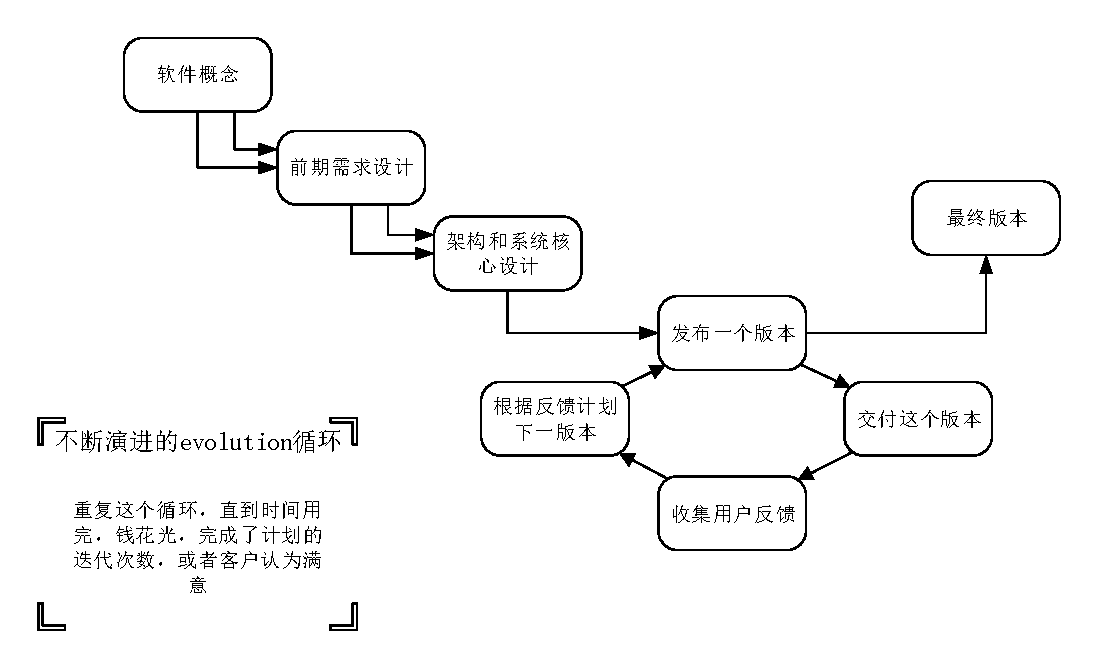
\includegraphics[width=0.9\columnwidth]{figures/system_development_process}
	%  \setlength{\abovecaptionskip}{0pt}
	%  \setlength{\belowcaptionskip}{-20pt}
	\caption{系统开发流程图}
	\label{fg:system_development_process}
\end{figure}

\subsection{用户体验}
用户体验评价标准:
\begin{table}[H]
  \centering
  \caption{用户体验评价标准}
    \begin{tabular}{|p{8.335em}|p{17.665em}|}
    \hline
    \textcolor[rgb]{ .298,  .282,  .239}{评价标准} & \textcolor[rgb]{ .298,  .282,  .239}{评价要求} \\
    \hline
    \textcolor[rgb]{ .298,  .282,  .239}{尽快提供可感触的反馈} & \textcolor[rgb]{ .298,  .282,  .239}{系统状态要有反馈,等待时间要合适} \\
    \hline
    \textcolor[rgb]{ .298,  .282,  .239}{系统界面符合用户的现实惯例} & \textcolor[rgb]{ .298,  .282,  .239}{与用户沟通使用用户语言而不是开发者语言,给用户提供必要的信息提示,减少用户的记忆负担,从而减少认知阻力} \\
    \hline
    \textcolor[rgb]{ .298,  .282,  .239}{用户有控制权} & \textcolor[rgb]{ .298,  .282,  .239}{操作失误可以回退,要让用户可以退出软件,用户可以定制显示信息的多少,还可以定制常用设置} \\
    \hline
    \textcolor[rgb]{ .298,  .282,  .239}{一致性和标准化} & \textcolor[rgb]{ .298,  .282,  .239}{对同一事物和同类操作的表示用语,各处要保持一致} \\
    \hline
    \textcolor[rgb]{ .298,  .282,  .239}{适合各种类型的用户} & \textcolor[rgb]{ .298,  .282,  .239}{要为新手和专家提供可定制化的设计,对于长期使用软件的用户,应该能够适应用户的使用习惯,让用户越用越顺手,最后产生感情上的好感和忠诚度} \\
    \hline
    \multirow{2}[2]{*}{\textcolor[rgb]{ .298,  .282,  .239}{帮助用户识别、诊断并修复错误}} & \textcolor[rgb]{ .298,  .282,  .239}{软件的关键操作要有确认提示,以便帮助用户及早消除误操作。要注意使用朴素的语言描述错误信息,错误信息要给出下一步操作提示。} \\
    \multicolumn{1}{|c|}{} & \textcolor[rgb]{ .298,  .282,  .239}{让所有的用户都可以通过电子邮件或者表单来提交反馈意见} \\
    \hline
    \textcolor[rgb]{ .298,  .282,  .239}{有必要的提示和帮助文档} & \textcolor[rgb]{ .298,  .282,  .239}{必要时提供在线帮助和帮助文档} \\
    \hline
    \end{tabular}%
  \label{tab:yhty}%
\end{table}%


\subsection{软件测试和质量保障}
\subsubsection{软件测试}\

在软件开发过程中的每一个小阶段都要进行当前已经完成的软件的测试,测试需要测试文档,包括测试设计说明书,测试用例,程序错误报告和测试报告。其中测试报告中需要按照如下要求报告bug:

\paragraph{症状:}\

即从用户的角度看,软件出了什么问题。

\paragraph{程序错误:}\

即从代码的角度看,软件的什么错误导致了软件的问题。

\paragraph{根本原因:}\

错误根源,即导致代码错误的根本原因。

\begin{figure}[H]
	\centering
	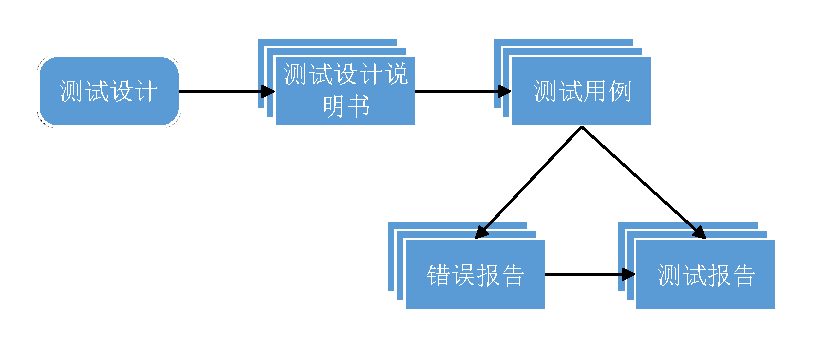
\includegraphics[width=0.9\columnwidth]{figures/test_document}
	%  \setlength{\abovecaptionskip}{0pt}
	%  \setlength{\belowcaptionskip}{-20pt}
	\caption{测试工作中的文档}
	\label{fg:test_document}
\end{figure}

\subsubsection{质量保障}\

成立软件质量保证(SQA)小组,确保开发者确实进行高质量的工作,每个开发者和维护者应对检查自己工作正确负责,每一个阶段性的工作完成之后由SQA小组审查工作的正确性和完整性,每一个阶段性的工作完成之后由SQA小组审查对应文档的完整性。

\begin{figure}[H]
	\centering
	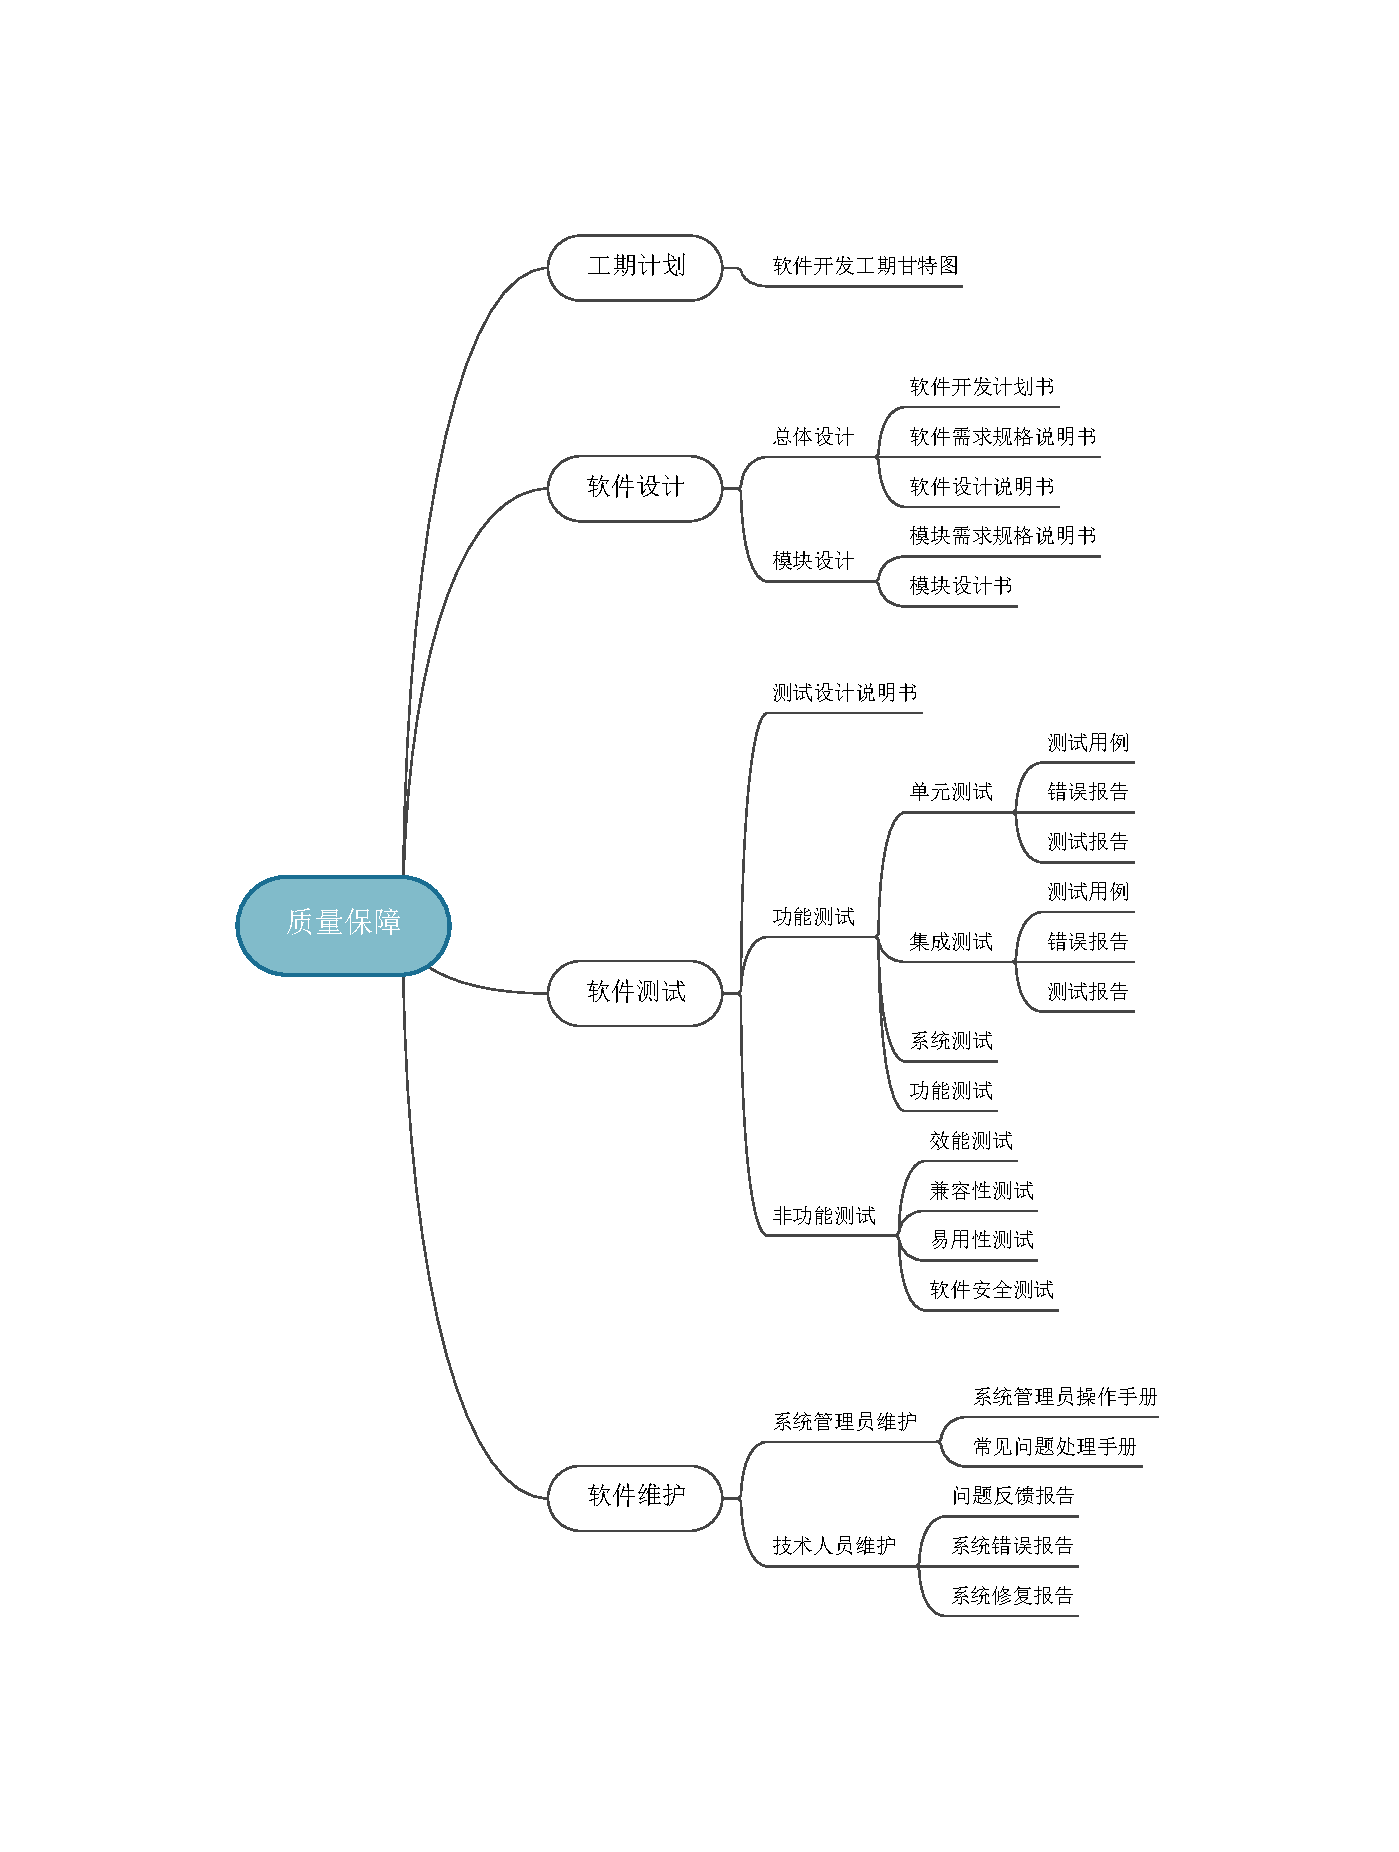
\includegraphics[width=0.9\columnwidth]{figures/software_quality_assurance}
	%  \setlength{\abovecaptionskip}{0pt}
	%  \setlength{\belowcaptionskip}{-20pt}
	\caption{软件质量保障文档审核总览}
	\label{fg:software_quality_assurance}
\end{figure}

\subsection{成本估算}
\subsubsection{硬件成本}\

以华为云在2018年6月30号的价格报表为参考标准,最终租赁版本未确定。

% Table generated by Excel2LaTeX from sheet 'Sheet1'
\begin{table}[H]
  \centering
  \caption{硬件成本估计}
    \begin{tabular}{|p{4.055em}|p{5.555em}cc|}
    \hline
    \textcolor[rgb]{ .298,  .282,  .239}{租赁项目} & \multicolumn{1}{p{5.555em}|}{\textcolor[rgb]{ .298,  .282,  .239}{服务器}} & \multicolumn{1}{p{5.72em}|}{\textcolor[rgb]{ .298,  .282,  .239}{云存储}} & \multicolumn{1}{p{5.835em}|}{\textcolor[rgb]{ .298,  .282,  .239}{分布式存储预留}} \\
    \hline
    \textcolor[rgb]{ .298,  .282,  .239}{成本(元)} & \multicolumn{1}{p{5.555em}|}{\textcolor[rgb]{ .298,  .282,  .239}{2998.80/年}} & \multicolumn{1}{p{5.72em}|}{\textcolor[rgb]{ .298,  .282,  .239}{2652.00/年}} & \multicolumn{1}{p{5.835em}|}{\textcolor[rgb]{ .298,  .282,  .239}{5000/年}} \\
    \hline
    \textcolor[rgb]{ .298,  .282,  .239}{总计(元)} & \multicolumn{3}{p{17.11em}|}{\textcolor[rgb]{ .298,  .282,  .239}{10650.8/年}} \\
    \hline
    \end{tabular}%
  \label{tab:yjcb}%
\end{table}%


\subsubsection{人力成本}\

系统开发周期为1个月,人员初定为6人(美工1人,服务器搭建1人,视频底层工程师1人,网页工程师1人,Android and iOS工程师2人)。考虑工程开发实际情况,预留金额20000元,用于人员扩充与激励措施。

% Table generated by Excel2LaTeX from sheet 'Sheet1'
\begin{table}[H]
  \centering
  \caption{人力成本预计}
    \begin{tabular}{|p{4.055em}|cccccc|}
    \hline
    \textcolor[rgb]{ .298,  .282,  .239}{职位} & \multicolumn{1}{p{4.055em}|}{\textcolor[rgb]{ .298,  .282,  .239}{美工}} & \multicolumn{1}{p{5em}|}{\textcolor[rgb]{ .298,  .282,  .239}{服务器搭建}} & \multicolumn{1}{p{4.055em}|}{\textcolor[rgb]{ .298,  .282,  .239}{视频底层工程师}} & \multicolumn{1}{p{4.165em}|}{\textcolor[rgb]{ .298,  .282,  .239}{网页工程师}} & \multicolumn{1}{p{5.665em}|}{\textcolor[rgb]{ .298,  .282,  .239}{Android \& iOS工程师}} & \multicolumn{1}{p{4.055em}|}{\textcolor[rgb]{ .298,  .282,  .239}{预留资金}} \\
    \hline
    \textcolor[rgb]{ .298,  .282,  .239}{人数} & \multicolumn{1}{c|}{\textcolor[rgb]{ .298,  .282,  .239}{1}} & \multicolumn{1}{c|}{\textcolor[rgb]{ .298,  .282,  .239}{1}} & \multicolumn{1}{c|}{\textcolor[rgb]{ .298,  .282,  .239}{1}} & \multicolumn{1}{c|}{\textcolor[rgb]{ .298,  .282,  .239}{1}} & \multicolumn{1}{c|}{\textcolor[rgb]{ .298,  .282,  .239}{2}} & \multirow{2}[4]{*}{\textcolor[rgb]{ .298,  .282,  .239}{20000}} \\
\hline{1-6}    \textcolor[rgb]{ .298,  .282,  .239}{酬薪(元\textbackslash{}人\textbackslash{}月)} & \multicolumn{1}{c|}{\textcolor[rgb]{ .298,  .282,  .239}{6000}} & \multicolumn{1}{c|}{\textcolor[rgb]{ .298,  .282,  .239}{20000}} & \multicolumn{1}{c|}{\textcolor[rgb]{ .298,  .282,  .239}{10000}} & \multicolumn{1}{c|}{\textcolor[rgb]{ .298,  .282,  .239}{10000}} & \multicolumn{1}{c|}{\textcolor[rgb]{ .298,  .282,  .239}{12000}} &  \\
    \hline
    \textcolor[rgb]{ .298,  .282,  .239}{总计(元)} & \multicolumn{6}{c|}{\textcolor[rgb]{ .298,  .282,  .239}{90000}} \\
    \hline
    \end{tabular}%
  \label{tab:rlcb}%
\end{table}%


\subsubsection{项目开发预计总成本}\

% Table generated by Excel2LaTeX from sheet 'Sheet1'
\begin{table}[H]
  \centering
  \caption{项目开发总成本}
    \begin{tabular}{|p{5em}|cc|}
    \hline
    \multicolumn{1}{|r|}{\textcolor[rgb]{ .298,  .282,  .239}{}} & \multicolumn{1}{p{4.055em}|}{\textcolor[rgb]{ .298,  .282,  .239}{硬件成本}} & \multicolumn{1}{p{4.055em}|}{\textcolor[rgb]{ .298,  .282,  .239}{人力成本}} \\
    \hline
    \textcolor[rgb]{ .298,  .282,  .239}{资金(元)} & \multicolumn{1}{c|}{\textcolor[rgb]{ .298,  .282,  .239}{10650.8}} & \textcolor[rgb]{ .298,  .282,  .239}{90000} \\
    \hline
    \textcolor[rgb]{ .298,  .282,  .239}{总计(元)} & \multicolumn{2}{c|}{\textcolor[rgb]{ .298,  .282,  .239}{100650.8}} \\
    \hline
    \end{tabular}%
  \label{tab:kfzcb}%
\end{table}%


\subsubsection{时间成本}\

开发周期约一个月,团队成员6人。







%研发概况
%\section{公司}
\subsection{公司名称}
一课,缩写为ike(Internet Knowledge and Experience)。知识改变命运。
\subsection{公司简介}
\subsubsection{公司性质}\

有限责任公司
\subsubsection{公司理念}\

核心价值观是企业文化的灵魂,是企业的特质,是行动的准则,也是我们共同的信念。它使企业有了互信互谅的工作氛围,使企业有了创新变革的前进勇气,使企业有了合作共赢的奋斗理想,使企业有了争做第一的远景展望。我们创业团队的核心价值观就是:善于学习,勇于创新,团结协作,服务大众。

本公司将把核心价值观渗透到公司的日常管理中,使以企业核心价值观为中心的企业文化成为每个人坚定的信念,使企业核心价值观贯彻在每个人的一言一行、一举一动中,使核心价值观溶化在每一个人的血液里,使企业核心价值观体现在战略思考、战略执行的结果中,这将是我们始终如一的信念。

\subsubsection{公司目标}\

本公司将持续不断的健全管理机制,培育核心技术能力,建立竞争优势,增强自我完善和自我发展的能力;同时我们会履行社会责任,服务于社会、回报于社会,为整个价值链系统创造最大的价值;专心专意打造一流的在线教育平台,为产业创新的良性发展注入成功基因,整合优势的资源,为国家的进步、社会的创新做贡献。行为识别是企业识别系统(CIS)中的重要方面,是企业理念付诸于计划行为的方式。它是企业员工如何履行职责的行为规范。它在组织制度、管理培训、行为规则、公关礼仪等方面表现出来,使抽象的理念化为有形的行为,是我们在实际行动中的目标。在企业识别系统(CIS)中,行为识别有着最广泛的内容,这也是我们公司所期待达成的目标:
\paragraph{企业员工共同行为规范:}\

关心政治,善于学习 热爱企业,忠于职守

发扬传统,勇于创新 钻研业务,讲求效率

团结协作,遵章守纪 艰苦奋斗,厉行节约

\paragraph{企业管理人员行为规范:}\

政治坚定,诚信经营 发扬传统,勇于创新

科学管理,民主决策 维护团结,作风正派

勤俭节约,廉洁奉公 关心职工,联系群众

\subsection{公司控股结构}
%还没写啊!!!!!!!!!!!!!!!!!!!!!!!!!

\subsection{公司架构}
公司架构:
\begin{figure}[H]
	\centering
	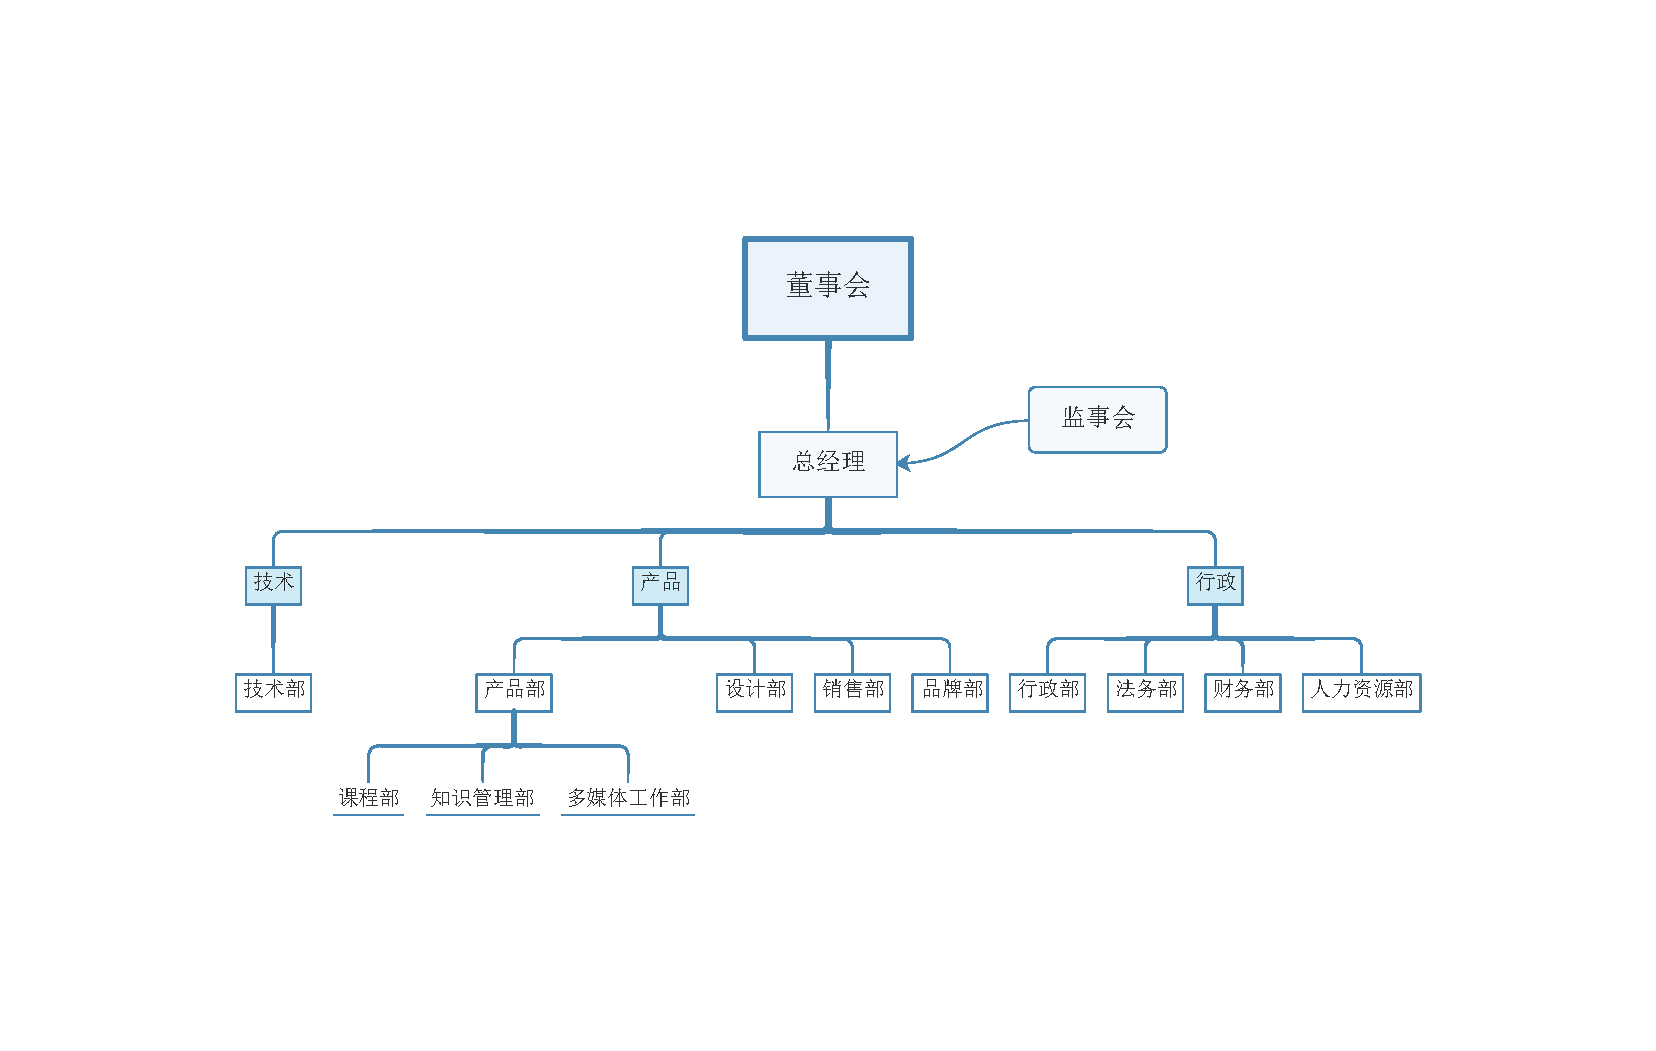
\includegraphics[width=0.9\columnwidth]{figures/management_layer}
	%  \setlength{\abovecaptionskip}{0pt}
	%  \setlength{\belowcaptionskip}{-20pt}
	\caption{公司架构图}
	\label{fg:management_layer}
\end{figure}

\subsubsection{管理层职责}\

主持公司全面工作,负责公司的全面领导和管理工作确定公司各部门分工及职权,确保公司各部门有序高效运转;

制定公司发展战略、发展计划和各项运营指标,全面把握公司的运营状况,并做出针对性调整决定;

负责把握公司业务的开展方向,与市场部、产品部、销售部等多部门协调制定公司业务暨课程内容的发展规划;

决定调整公司的组织结构、人员编制;决定公司干部的聘任、解聘、晋升和奖惩;
定期组织召开公司全体会议,检查、监督和协调各部门,各项目工作任务完成情况;

负责公司企业文化建设和员工理念、形象、素质建设,创造一流的公司品牌和公司形象;

负责公司重大项目的对外对接工作,保证公司项目运转顺利进行。

\subsection{主要业务}
\begin{itemize}
  \item 广播电视节目制作
  \item 互联网信息服务
  \item 从事互联网文化活动
  \item 出版物零售。技术开发、技术转让、技术咨询、技术服务
  \item 基础软件服务
  \item 应用软件服务
  \item 软件开发
  \item 教育咨询
  \item 组织文化艺术交流活动(不含营业性演出)
  \item 文化咨询
  \item 会议服务
  \item 承办展览展示活动
\end{itemize}


\subsection{员工组成}
课程运营人员、营销人员、系统运维人员、管理人员。

希望是全985、211高校(课程运营人员),若前期成本太高,公司可以请高校实习生,但技术人员需求专业人员或者科班出身,原因有以下三个方面:

\paragraph{节约第三方评价课程成本}\

如果公司本身就有这方面专业的高校学生,无论他学习是否好,至少他对于专业的了解是足够的,或者他直接认识专业知识非常优秀的人,或者其他同学或者师兄,师姐,老师,公司就不用再花钱去找人来评价我们不懂的课程内容了,在准确度方面也有相对较好的把握。

\paragraph{业务能力好,执行力强}\

员工组成大部分为高水平院校大学生群体,相对于其他公司人员业务能力将会更好,同时也具有更强的执行力。员工的业务能力、执行力等在一定程度上决定了公司发展的潜力,这一点对于公司的长久规划至关重要

\paragraph{人脉资源广,办事效率高}\

未来课程录制上教师选择会有许多不同需求,高水平院校大学生群体员工相对其他公司而言人脉资源更为广泛,在教师资源上将有更多选择且效率将会更高。这极大保障了公司产品的质量优势同时缩短了产品的研发周期

\subsection{公司发展目标}
公司发展理念:
\begin{figure}[H]
	\centering
	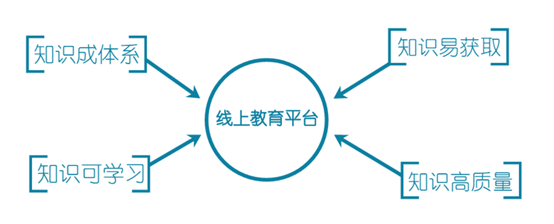
\includegraphics[width=0.9\columnwidth]{figures/company_development}%改成公司发展理念图
	%  \setlength{\abovecaptionskip}{0pt}
	%  \setlength{\belowcaptionskip}{-20pt}
	\caption{公司发展理念图}
	\label{fg:company_development}
\end{figure}

\subsubsection{近期目标}\

在公司发展前期,主要完成以下三方面任务:
\paragraph{系统研发}\

完成系统的研发工作,进行课程录制,达到一定数量后投放市场。课程需要包括视频、音频、文字这三种主要的知识载体。

\paragraph{需求调研}\

通过市场需求预调研有针对性录制迎合市场需求课程,通过校园代理或与线下机构合作的方式在短期内打开市场并实现部分盈利。课程录制的方向是:先进行市场调查,市场调查的依据是询问线下教育行业人士,然后针对性的进行课程录制,课程销售交给线下教育行业人士,获得收益分成。

\paragraph{用户积累}\

完成一定的用户资源积累,通过内容至上的核心竞争力赢得良好声誉为进一步打开市场做准备;实现部分资本回收,为下一步丰富平台资源、搭建完整课程体系做资金准备。

\begin{figure}[H]
	\centering
	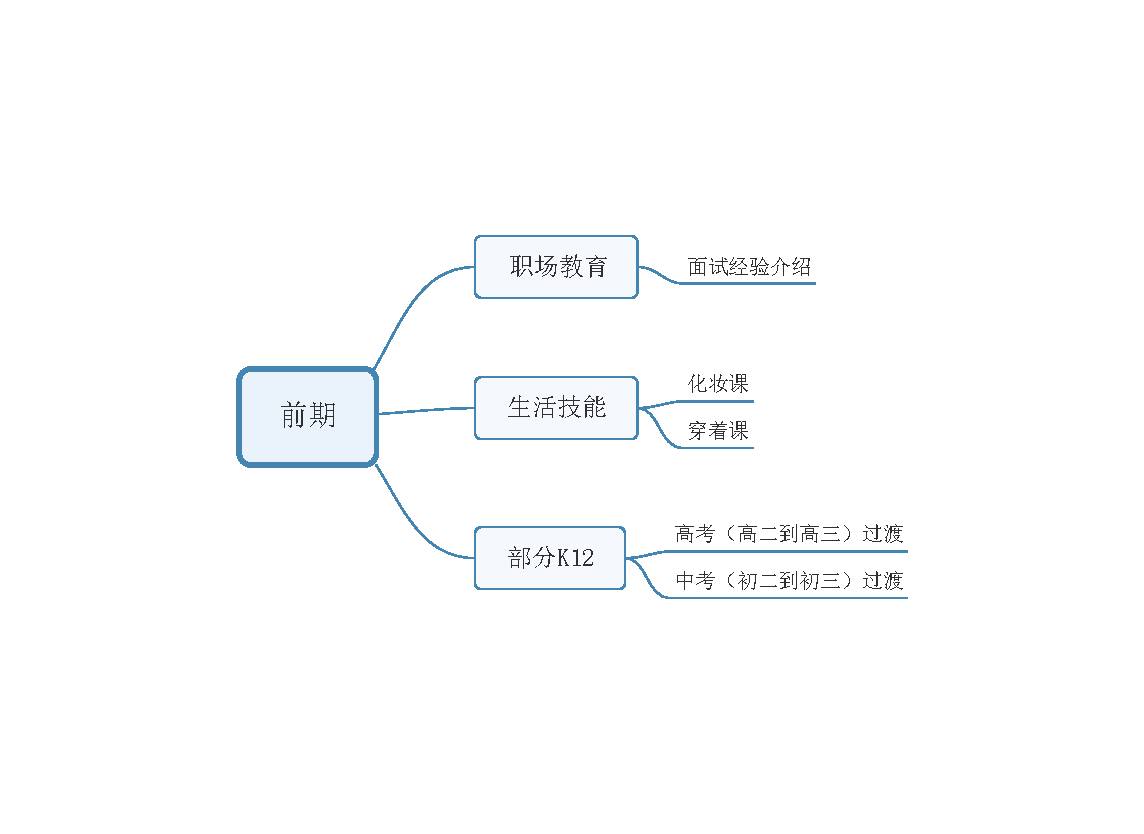
\includegraphics[width=0.9\columnwidth]{figures/prophase_development}%改图
	%  \setlength{\abovecaptionskip}{0pt}
	%  \setlength{\belowcaptionskip}{-20pt}
	\caption{前期课程发展图}
	\label{fg:prophase_development}
\end{figure}

\subsubsection{长期目标}\

在公司发展中期,主要完成以下六个方面任务:

\paragraph{增加销售人员}\

当前期盈利模式获得一定收益之后,增加销售部,销售部组成人员主要来源于社会招聘,通过市场上的有经验的销售人员,通过销售人员来留住客户。

\paragraph{课程录制转型}\

课程录制开始逐渐完善平台总体课程框架,课程录制从市场主导型转为“优先发展课程体系内市场迎合度高的产品”(市场倾向性),注重资本快速积累的同时关注长期目标实现。

\paragraph{增加品牌知名度}\

开始录制大学专业介绍类课程,同时部分课程免费开放,吸引更多用户流量以打开市场,初步拥有品牌知名度。

\paragraph{课程整合}\

对平台课程视频资源的重新整合加工,调整和优化课程内容,进一步从课程结构上提升产品质量,进一步提升产品用户活跃度与美誉度。知识管理部门初创。

\paragraph{搭建课程框架}\

涉足高等教育、从业资格教育、成人教育中部分内容,初步搭建公司全品类教育框架,在同类平台中拥有一定市场竞争力。

\paragraph{加大融资}\

进一步加大融资力度,助力公司长远发展。
\newpage
\begin{figure}[H]
	\centering
	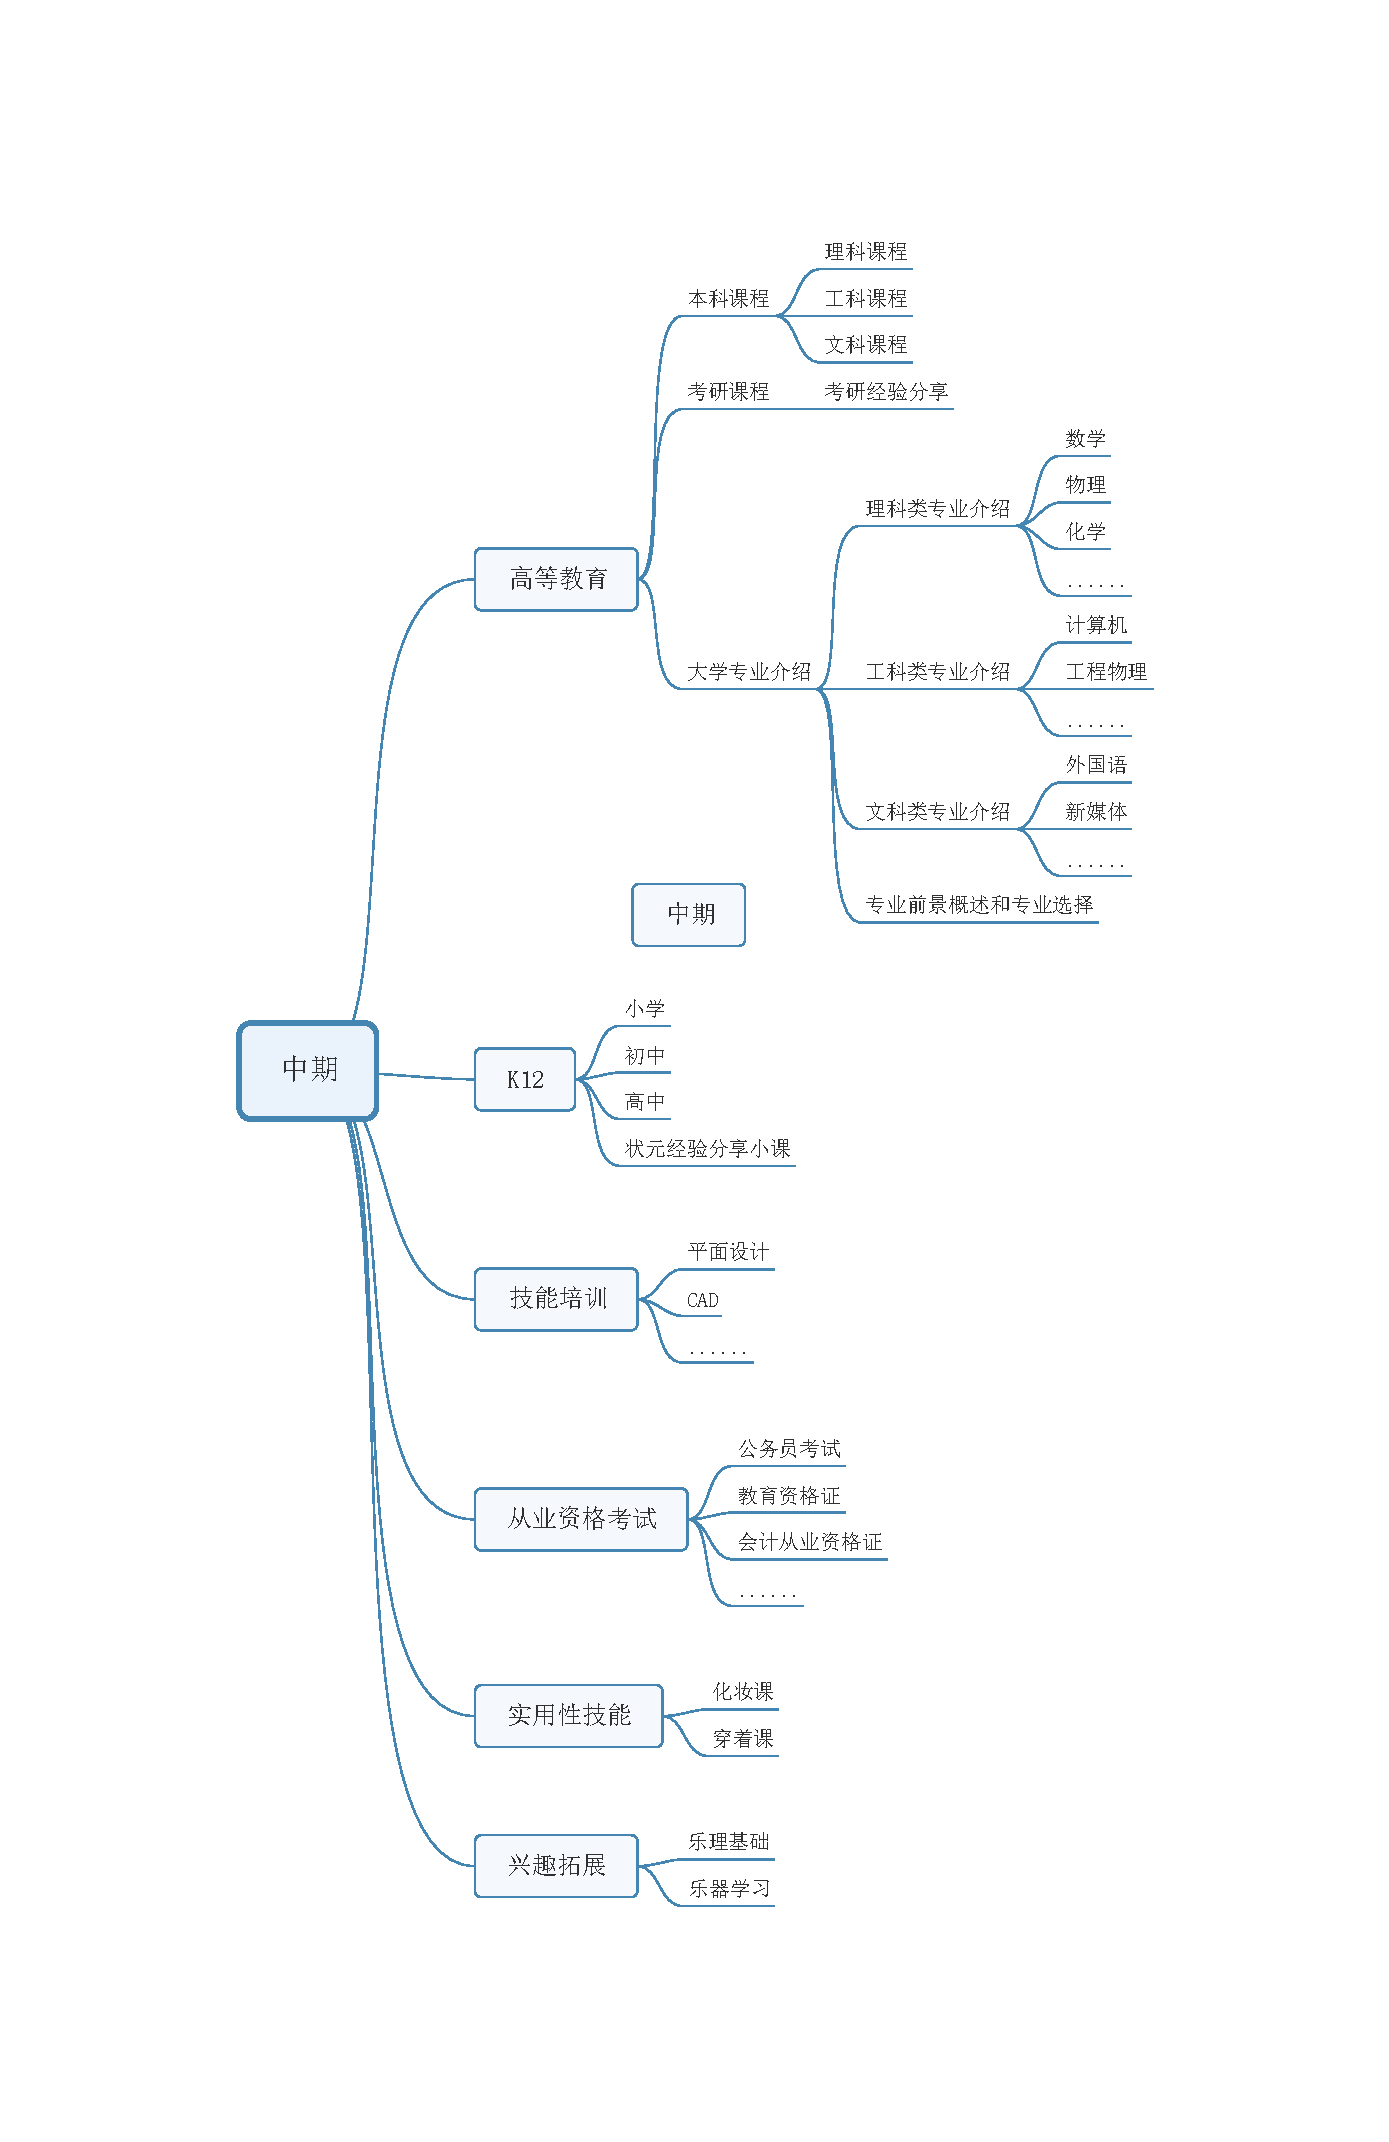
\includegraphics[width=10cm,height=17cm]{figures/mid_development}%改
	%  \setlength{\abovecaptionskip}{0pt}
	%  \setlength{\belowcaptionskip}{-20pt}
	\caption{中期课程发展图}
	\label{fg:mid_development}
\end{figure}

在公司的发展后期,我们主要完成以下任务:

\paragraph{占据较大市场份额}\

公司在在线教育行业拥有良好知名度和影响力,公司产品占据较大市场份额,资本积累达到一定高度。

\paragraph{完善课程体系}\

产品发展方向由市场倾向性变为课程体系主导型,进一步完善初始规划的课程体系,实现体系的专业性及完整性。

\paragraph{拓宽业务渠道}\

以在线教育为基础,向公司相关性产业如VR眼镜等进军,进一步拓宽业务渠道,扩大公司发展前景,增强公司生命力。

\paragraph{与政府合作}\

进军K12领域与地方政府合作,通过低价格的形式将课程卖给或者送给偏远贫困地区学生,打响平台品牌,践行公司社会责任、提升社会效益。

\paragraph{与高校合作}\

高等教育领域与高等教育院校合作,搭建高等教育知识传播平台,增强公司社会影响力,为中国人才培养提供长久而有力的支持。

\paragraph{主要盈利模式的转变}\

知识管理部门,以及公司知识创造过程的完善,以公司较完善的基础课程体系为基础,进行知识的二次加工创造,实现一个知识创造的循环。知识创造的输出以及对整个知识体系的构建,知识拓扑图的形成,对公司的产品来源、宣传上提供支持,逐渐转移主要盈利方向。

\begin{figure}[H]
	\centering
	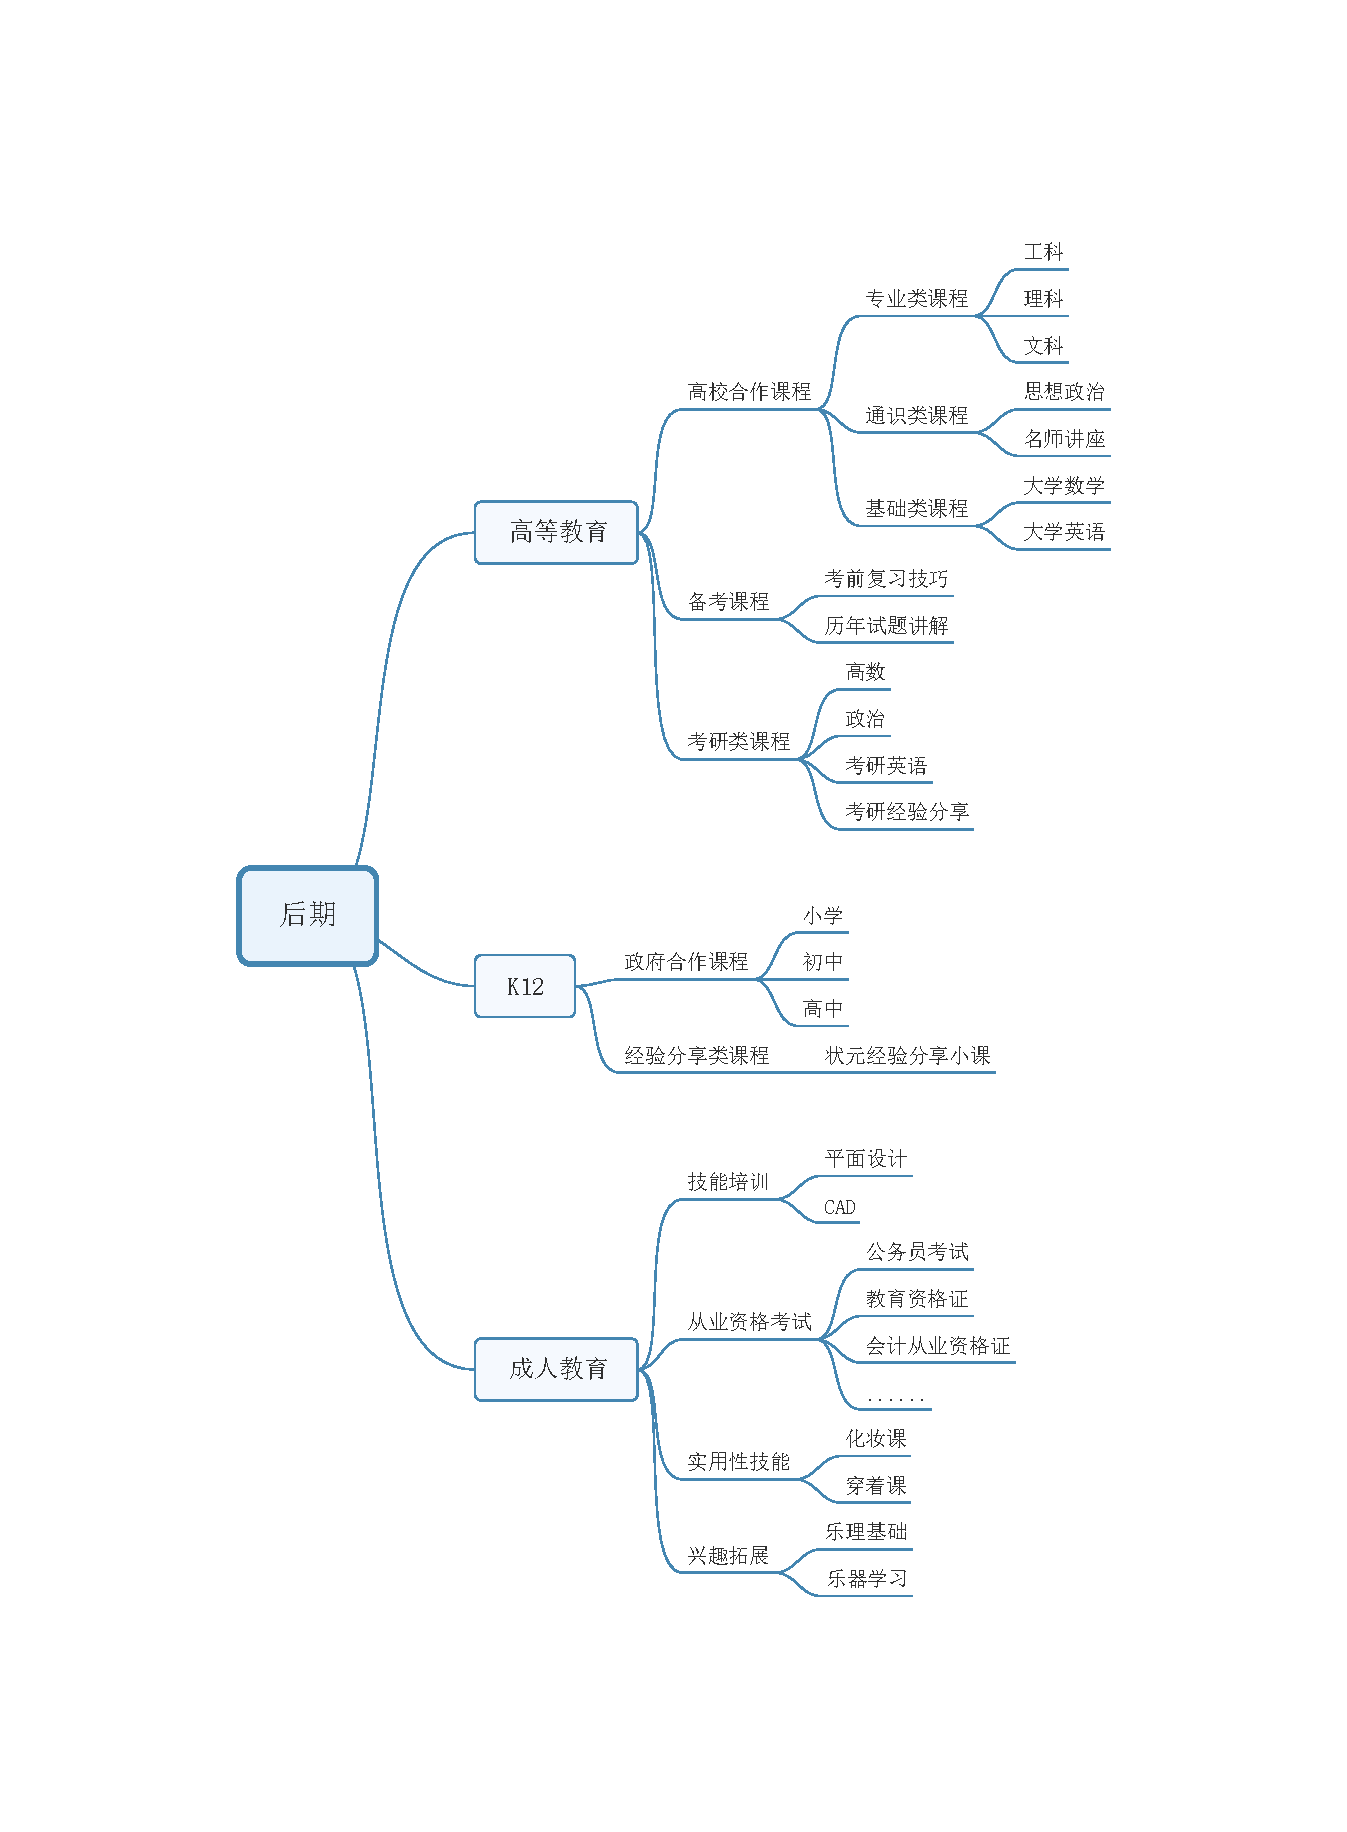
\includegraphics[width=0.9\columnwidth]{figures/aft_development}%改
	%  \setlength{\abovecaptionskip}{0pt}
	%  \setlength{\belowcaptionskip}{-20pt}
	\caption{后期课程发展图}
	\label{fg:aft_development}
\end{figure}

\subsection{三年规划五年目标}
三年内发展成为行业知名,具有一定市场影响力企业;五年内成为在线教育行业的引领者、市场规则的制定者,在追求经济效益的同时践行公司的社会责任。

\subsection{公司文化}
做一个服务用户的合作者,为有志青年提供知识改变命运的途径;

做一个理想的知识获取平台,为人才培养提供支持;

做网络知识领域的一面旗帜,为知识创新提供长远的推动力。

来一课,选择适合你的一课

这一课,不错过。














%公司
%\section{公司管理概况}
\subsection{高层简介}

\begin{table}[H]
  \centering
  \caption{高层简介}
    \begin{tabular}{|c|c|c|}
    \hline
    \textcolor[rgb]{ .298,  .282,  .239}{姓名} & \textcolor[rgb]{ .298,  .282,  .239}{学历} & \textcolor[rgb]{ .298,  .282,  .239}{专业} \\
    \hline
    \textcolor[rgb]{ .298,  .282,  .239}{陈洪璞} & \textcolor[rgb]{ .298,  .282,  .239}{中国人民大学本科在读} & \textcolor[rgb]{ .298,  .282,  .239}{信息管理与信息系统} \\
    \hline
    \textcolor[rgb]{ .298,  .282,  .239}{汪圣灵} & \textcolor[rgb]{ .298,  .282,  .239}{北京航空航天大学本科在读} & \textcolor[rgb]{ .298,  .282,  .239}{计算机科学与技术} \\
    \hline
    \textcolor[rgb]{ .298,  .282,  .239}{汪军水} & \textcolor[rgb]{ .298,  .282,  .239}{清华大学本科在读} & \textcolor[rgb]{ .298,  .282,  .239}{工程物理} \\
    \hline
    \end{tabular}%
  \label{tab:gaocengjeshao}%
\end{table}%

\subsection{高层分工}
高层分工如下:
\begin{figure}[H]
	\centering
	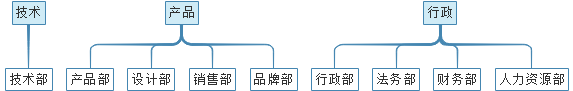
\includegraphics[width=0.9\columnwidth]{figures/high_level_division}
	%  \setlength{\abovecaptionskip}{0pt}
	%  \setlength{\belowcaptionskip}{-20pt}
	\caption{高层分工}
	\label{fg:high_level_division}
\end{figure}

\subsection{管理体系}
\subsubsection{课程管理体系}\

\paragraph{兼职课程运营管理}\

为开拓广阔的课程教师来源,我们公司会在必要的时期大量招收实习生,对兼职找老师的同学,我们的要求是要有一定的学生工作经验,若表现出色,则考虑吸收到创业团队。

\paragraph{课程教师管理}\

对课程教师,我们计划的筛选比例是20:1,同时为防止教师与其他在线教育平台合作,我们考虑两种方式,一种找专业非常好的大学在读生,未来就业方向不在教育领域,避免了冲突与竞争,第二种,课程收益与老师分成的形式,长期留住优秀的老师。若出现人气高的老师与其他在线教育平台合作,要第一时间找到可替代的老师。

\paragraph{课程制作时间控制}\

在课程市场调查结束之后,前期要预留一个月筛选老师,两个月进行宣传,保证有足够的时间应对突发情况。

\subsubsection{部门合作管理}\

各部门之间需要紧密合作,首先,以产品部为核心,产品部三大组成相互协调合作,共同规划产品方向与形式;以用户友好为目标,不断从课程品质和用户友好度方面完善平台产品。充分发挥高校兼职同学的创造力和想象力,同时,在法务和财务方面细化分工,防止出现意外情况。需要专人专职负责。

每周进行各部门理事会,每月部门负责人给全员汇报工作,统一思想。

\subsection{人事管理}
\subsubsection{管理思想}\

优良科学管理的前提是确定和贯彻正确先进的管理思想。我们将采取张瑞敏先生 “众谋独断、详虑力行”的管理思想。重视个人的发展,尊重个人价值, 但也同时强调各职能部门相互协调合作,求得公司的整体发展,实现最优效果。

\subsubsection{管理决策}\

公司初期的管理团队主要由创业团队人员组成。团队成员都是具本科在读的大学生,具有相关的专业知识和高效的执行力,将为公司制定切实可行的决策,执行最有效率的任务。在获得风险投资后,投资家自然也成为我们的公司管理顾问,我们还将邀请具有各专业技术及管理经验的人员加入,并担任重要职务。

\subsubsection{管理理念}\

关心员工成长、强化执行能力、追求高效和谐、平衡激励约束。

\paragraph{关心员工成长}\

重视员工的兴趣和专长,以良好的工作条件、完善的员工培训计划、职业生涯通道设计促进员工个人职业发展;重视企业文化管理,以健康简单的人际关系、严肃活泼的工作气氛、畅快透明的沟通方式,促进员工满意度的不断提高,使员工保持与企业同步成长的快乐;激发员工潜能,追求个人与公司共同成长。作为个人要有先付出的意识,甘于为团队奉献智慧和勤奋,以优秀的团队成就个人的优秀。
\paragraph{强化执行能力}\

再好的研究策划,没有好的执行就会成为空谈。强力执行是创业在管理上的核心原则之一;良好的执行力,要依靠优秀的机制、规范的制度、精诚的合作、有效的激励、感人的榜样,但最重要的,要依靠每位创业人对公司的热爱和对工作的负责精神;
\paragraph{追求高效和谐}\

根据公司发展阶段和业务变化,动态优化企业的管理,形成和谐有序的内部环境;在高效与和谐的环境下,坚持结果导向的管理原则,有效支持公司经营目标的实现。
\paragraph{平衡激励约束}\

根据工作贡献和成果价值, 形成差异化的激励机制,有效激发员工的主观能动性和创造性; 强调激励与约束相结合、保持平衡有度,为实现内部管理提供有力保障。

\paragraph{充分价值体现}\

充分发挥每一名员工的人脉资源与隐性知识,在人脉资源方面,配合课程部教师的合格找寻,成功介绍老师者将会有专门的奖励机制进行奖励;在个人隐性知识方面,充分体现员工优势,鼓励对显性知识的转化,同样有奖励机制。





%公司管理概况
%\section{投资回报}%投资回报
%\section{融资计划概述}
\begin{figure}[H]
	\centering
	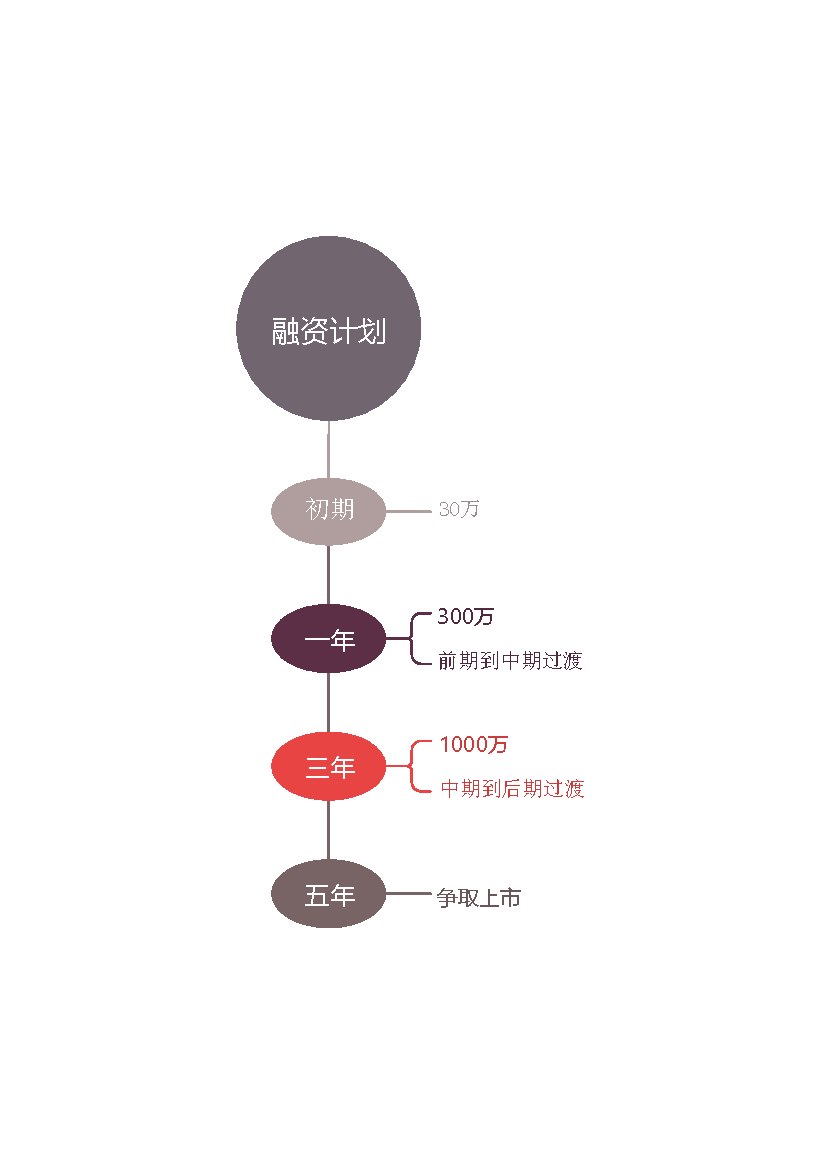
\includegraphics[width=8cm,height=13cm]{figures/rzjh}
	%  \setlength{\abovecaptionskip}{0pt}
	%  \setlength{\belowcaptionskip}{-20pt}
	\caption{融资计划概览图}
	\label{fg:rzjh}
\end{figure}%融资计划
%\section{风险概述}
\subsection{风险分类}

风险分为一下几类:
\begin{figure}[H]
	\centering
	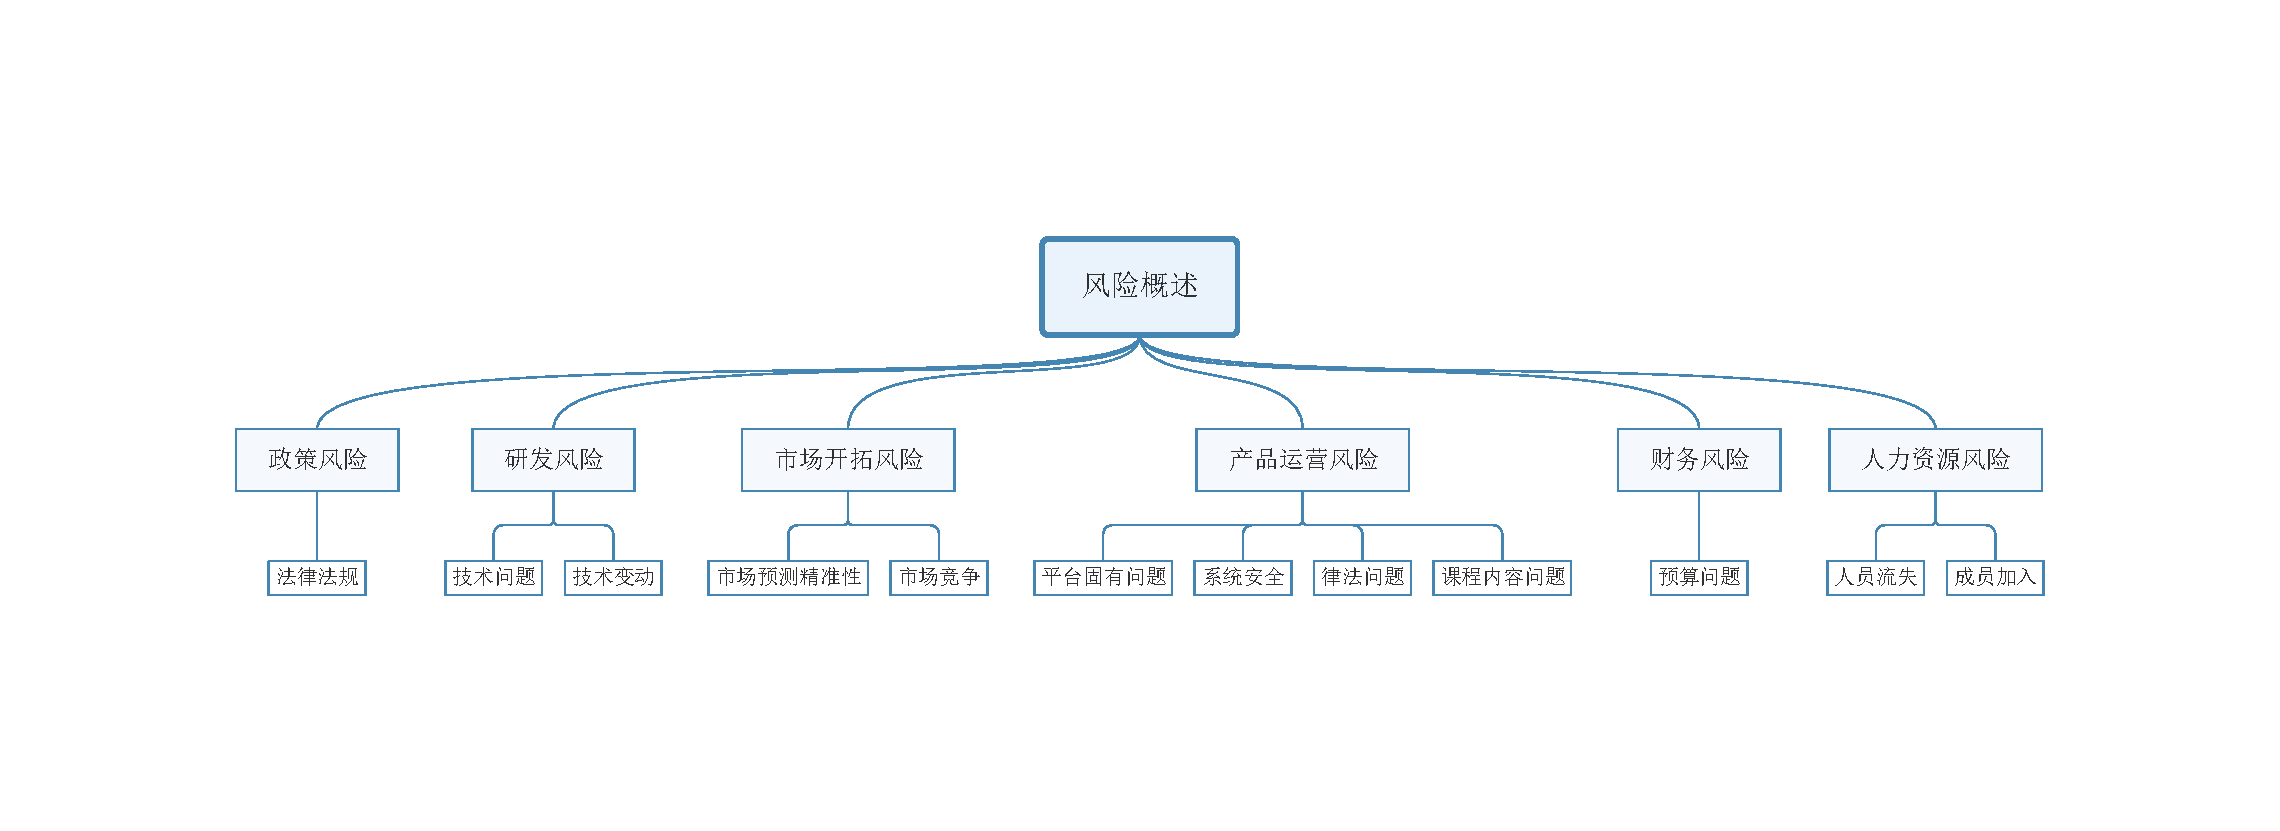
\includegraphics[width=0.9\columnwidth]{figures/risk_summary}
	%  \setlength{\abovecaptionskip}{0pt}
	%  \setlength{\belowcaptionskip}{-20pt}
	\caption{风险概述}
	\label{fg:risk_summary}
\end{figure}

\subsection{风险控制}

公司的创立与发展总是风险与机遇共存,想要发展成一个行业的领导者必定会面临各个方面带来的各种压力。所谓“知己知彼,百战不殆”,提前对可能遇到的风险做一个较为完全的预估是公司长久发展的基础。在充分考虑了政策、市场、产品运营、财务等各方面因素之后,本公司对发展中可能遇到的风险做了比较全面地评估,并提出了统一的风险控制模型以减少不必要的风险及可能带来的损失。

\begin{figure}[H]
	\centering
	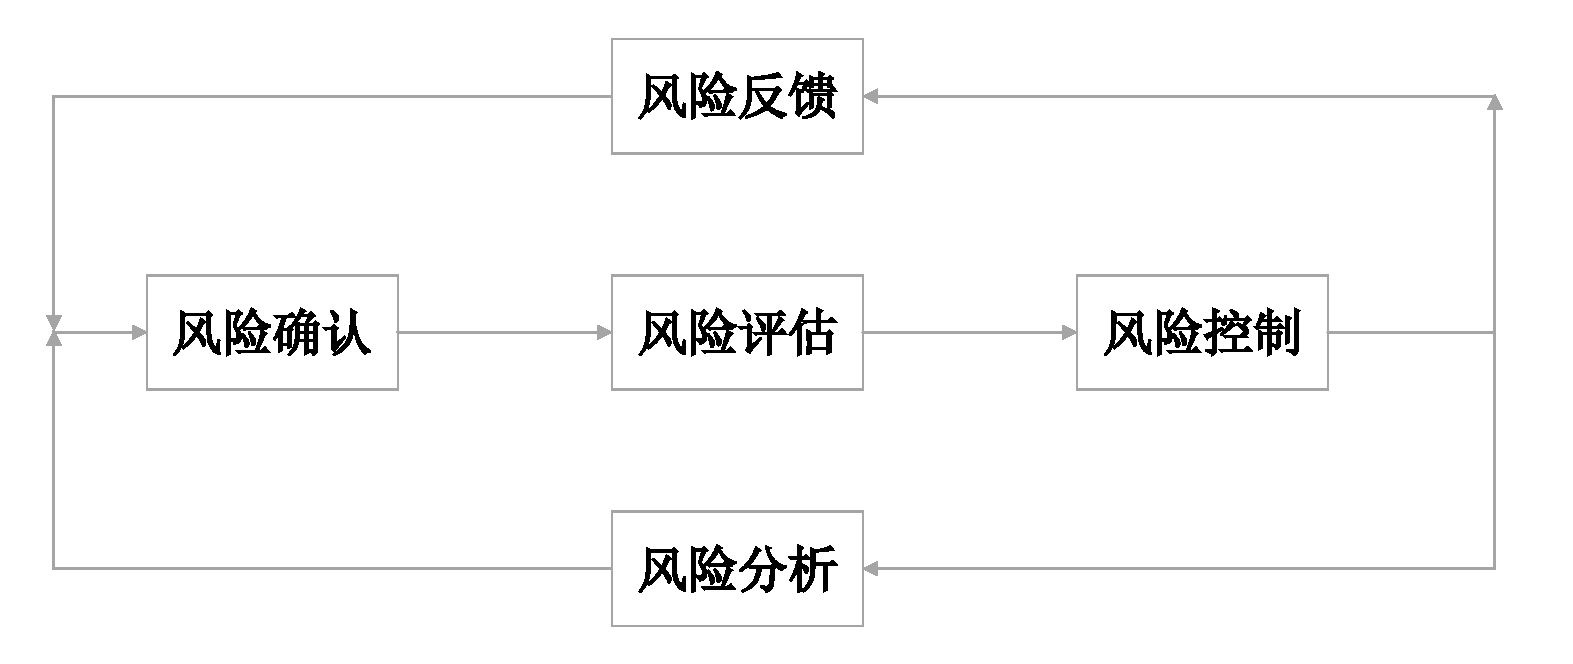
\includegraphics[width=0.9\columnwidth]{figures/rist_control}
	%  \setlength{\abovecaptionskip}{0pt}
	%  \setlength{\belowcaptionskip}{-20pt}
	\caption{风险控制}
	\label{fg:rist_control}
\end{figure}


\subsection{风险概览}
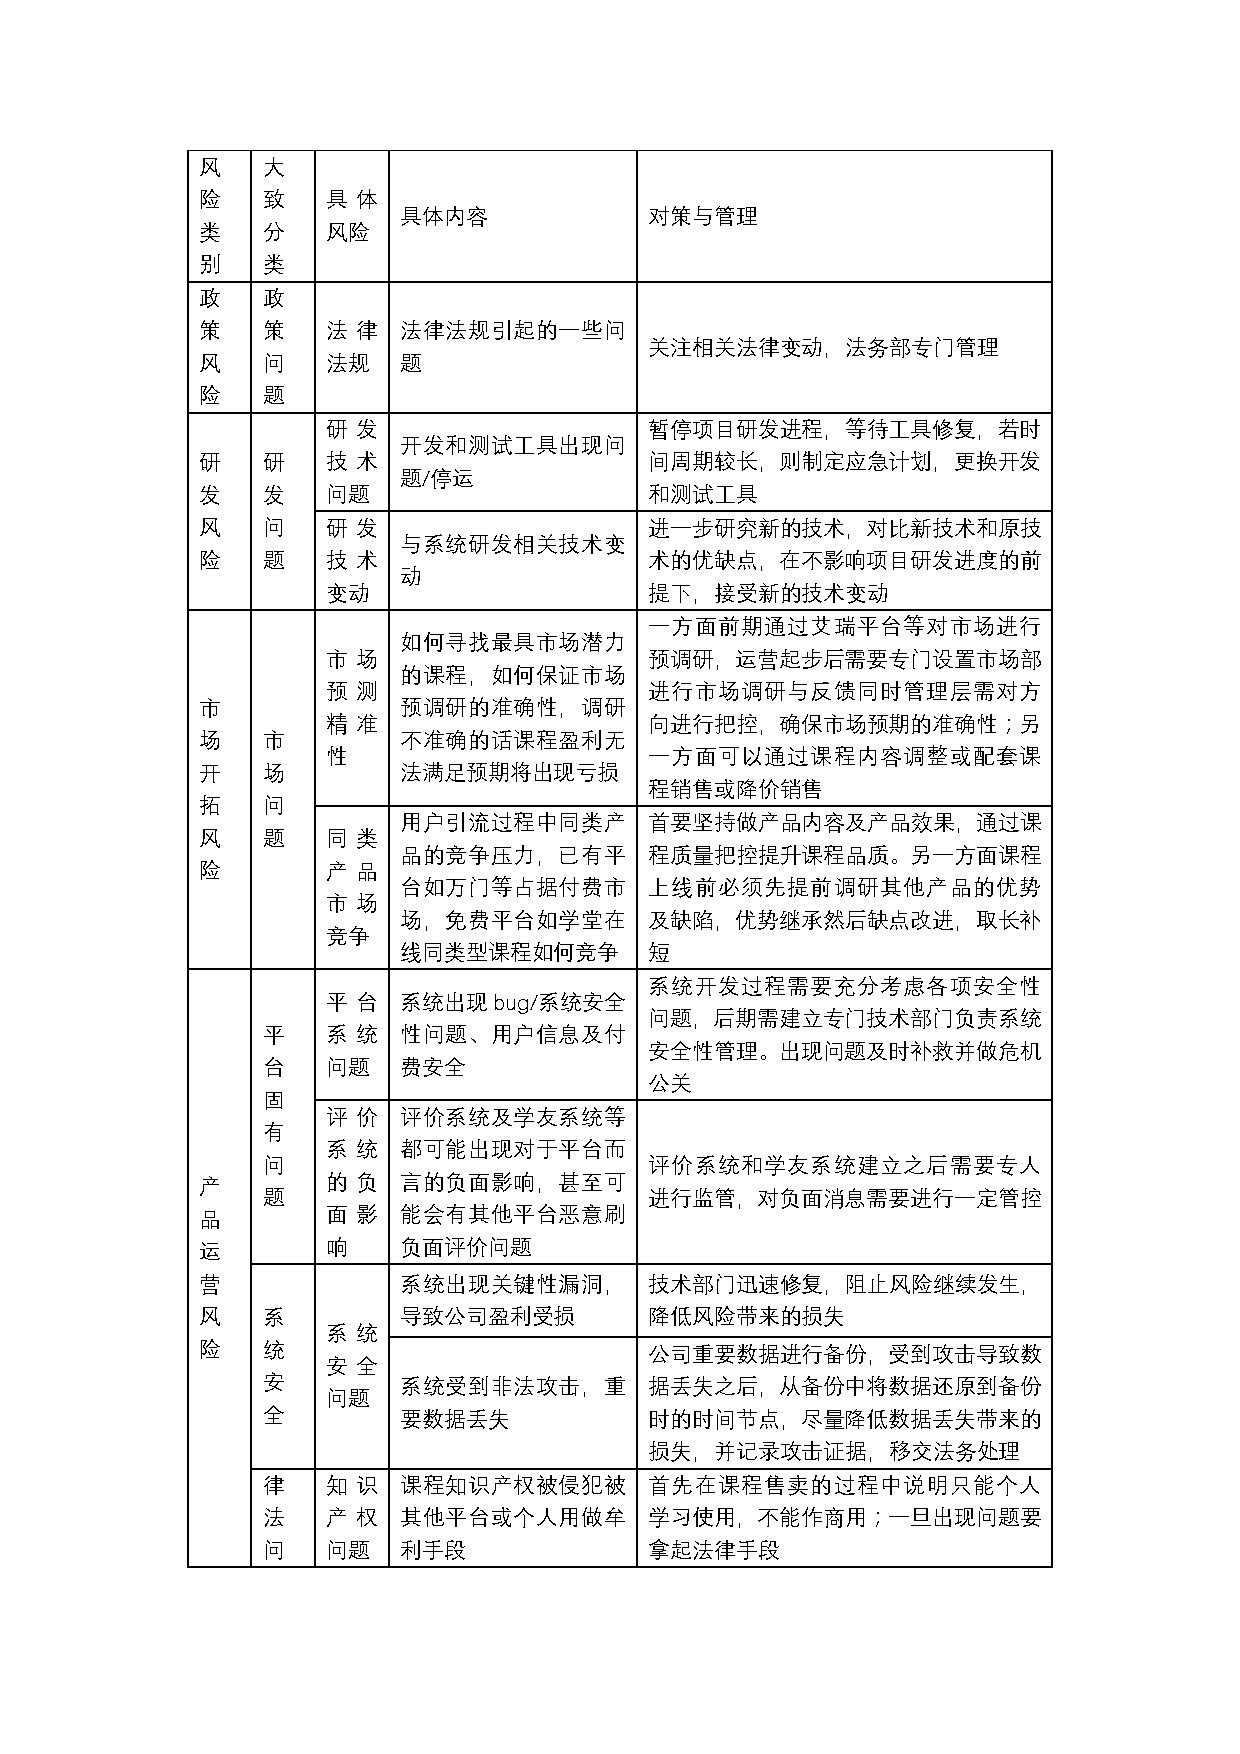
\includepdf{data/fxgs1.pdf}
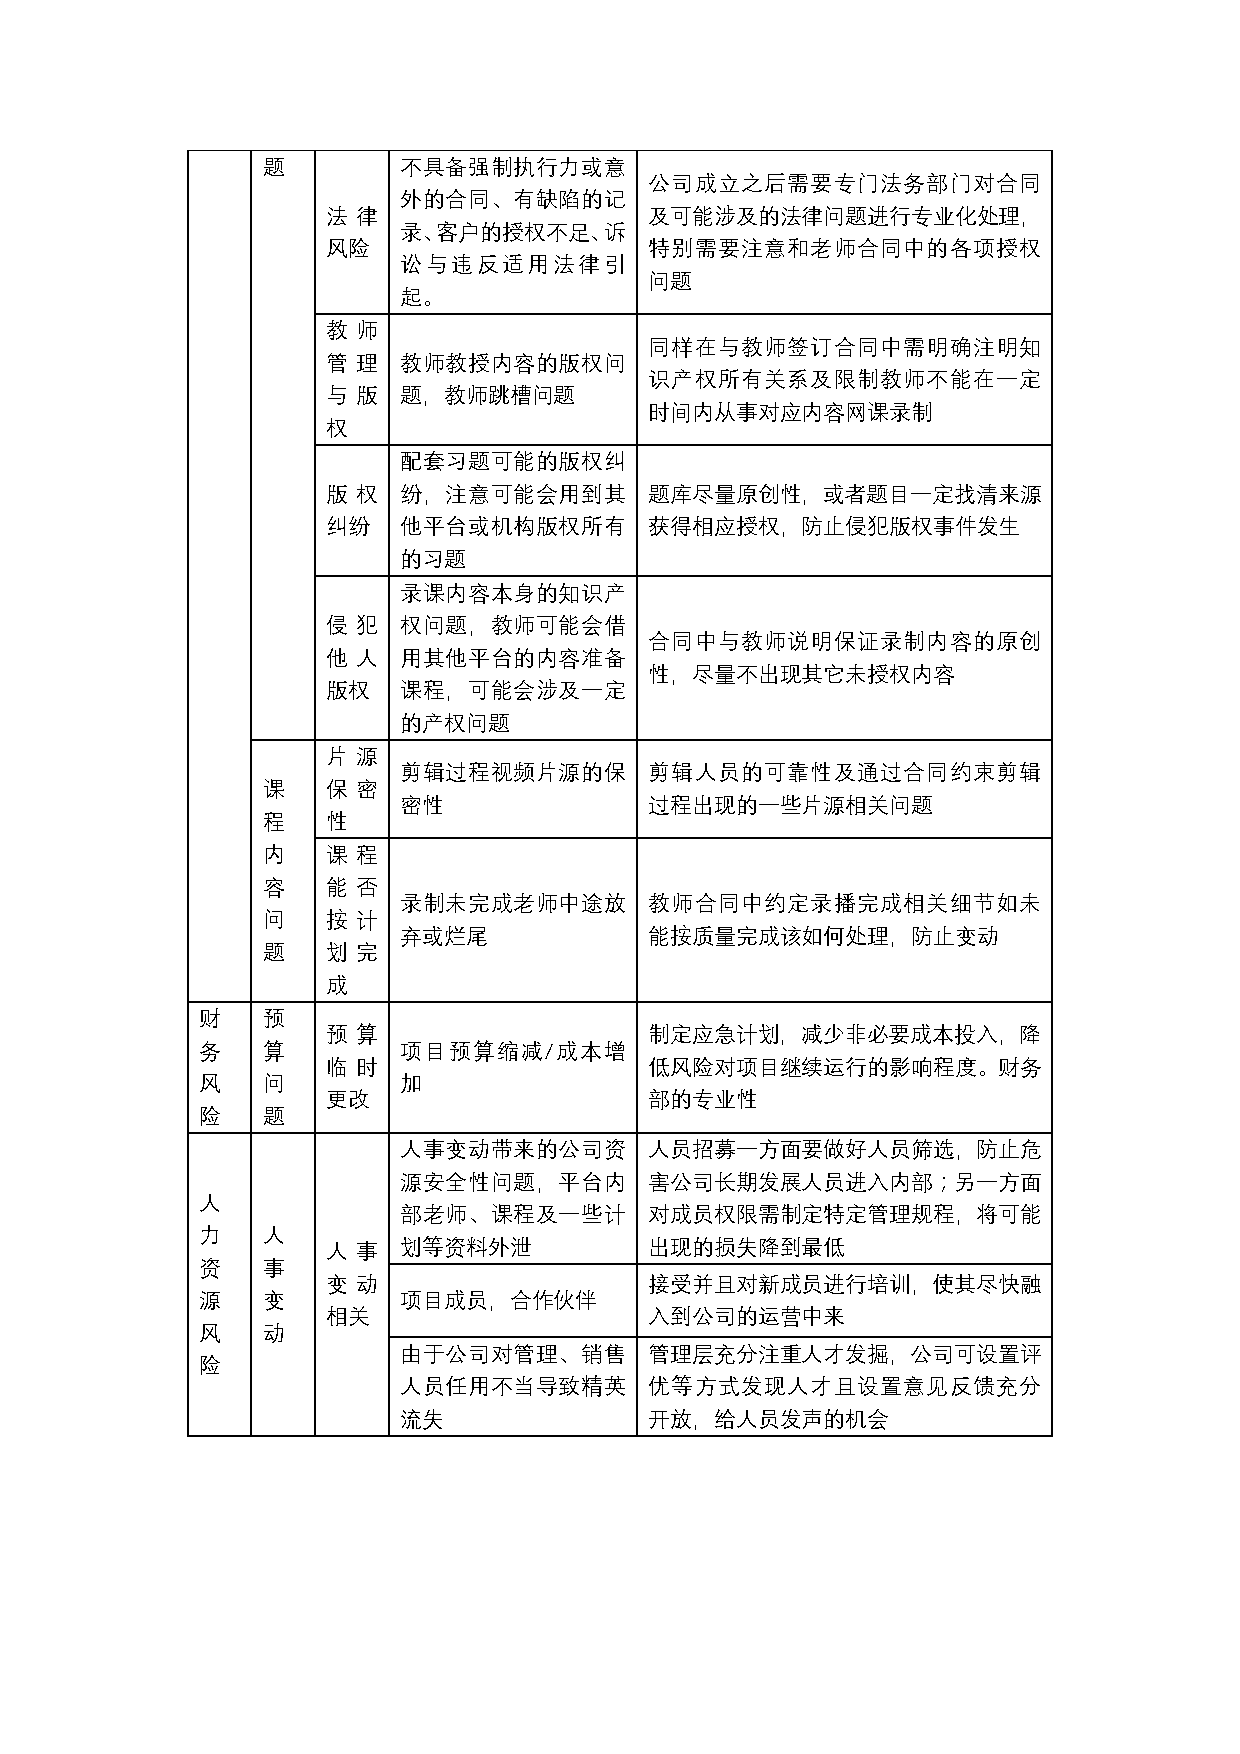
\includepdf{data/fxgs2.pdf}%风险概述
%\section{进度概览}
\begin{figure}[H]
	\centering
	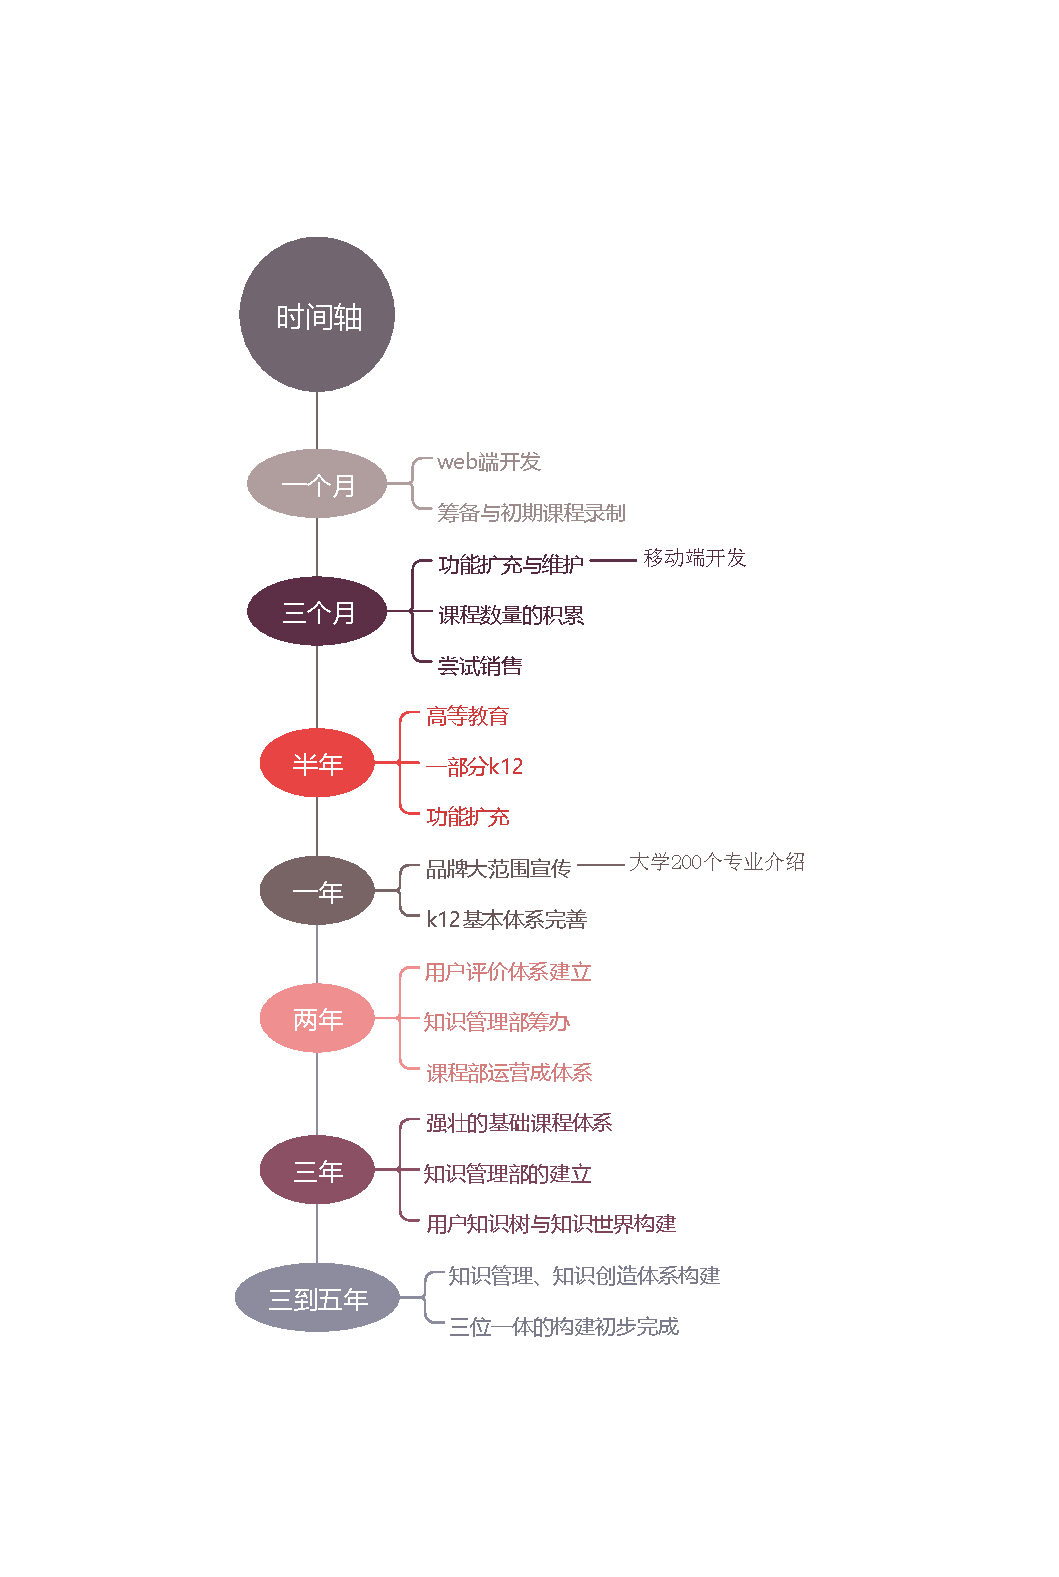
\includegraphics[width=8cm,height=13cm]{figures/jdb2}
	%  \setlength{\abovecaptionskip}{0pt}
	%  \setlength{\belowcaptionskip}{-20pt}
	\caption{总体进度概览图}
	\label{fg:jdb2}
\end{figure}%进度表
%book2
\section{摘要}
\subsection{产品简述}\ 
%段落开始,空一行为段落分段符



\subsection{策划结构综述}\ 
%段落开始,空一行为段落分段符

%摘要
\section{市场行业综述}
\subsection{历史发展}\ 
%段落开始,空一行为段落分段符


\subsection{现状}\ 
%段落开始,空一行为段落分段符

\subsection{前景}\ 
%段落开始,空一行为段落分段符

\subsection{结论总结}\ 
%段落开始,空一行为段落分段符%市场行业综述
\section{团队优势}
\subsection{团队成员介绍}\ 
%段落开始,空一行为段落分段符



\subsection{团队分工}\ 
%段落开始,空一行为段落分段符

%团队优势
\section{产品详细介绍}%主体部分
\subsection{产品服务}\ 
%段落开始,空一行为段落分段符


\subsection{盈利模式}\ 
%段落开始,空一行为段落分段符


\subsection{营销策略}\ 
%段落开始,空一行为段落分段符


\subsection{市场预测}\ 
%段落开始,空一行为段落分段符


\subsection{制作计划}\ %融资计划依据

\subsubsection{前期}\ %详细
%段落开始,空一行为段落分段符


\subsubsection{中期}\ %略
%段落开始,空一行为段落分段符


\subsubsection{后期}\ %略
%段落开始,空一行为段落分段符%产品详细介绍
\section{公司介绍}


%公司介绍
\section{融资计划}
%融资计划
\section{投资回报}


%投资回报

\newpage
\end{document}
